\batchmode
\documentclass[twoside]{book}

% Packages required by doxygen
\usepackage{fixltx2e}
\usepackage{calc}
\usepackage{doxygen}
\usepackage[export]{adjustbox} % also loads graphicx
\usepackage{graphicx}
\usepackage[utf8]{inputenc}
\usepackage{makeidx}
\usepackage{multicol}
\usepackage{multirow}
\PassOptionsToPackage{warn}{textcomp}
\usepackage{textcomp}
\usepackage[nointegrals]{wasysym}
\usepackage[table]{xcolor}

% Font selection
\usepackage[T1]{fontenc}
\usepackage[scaled=.90]{helvet}
\usepackage{courier}
\usepackage{amssymb}
\usepackage{sectsty}
\renewcommand{\familydefault}{\sfdefault}
\allsectionsfont{%
  \fontseries{bc}\selectfont%
  \color{darkgray}%
}
\renewcommand{\DoxyLabelFont}{%
  \fontseries{bc}\selectfont%
  \color{darkgray}%
}
\newcommand{\+}{\discretionary{\mbox{\scriptsize$\hookleftarrow$}}{}{}}

% Page & text layout
\usepackage{geometry}
\geometry{%
  a4paper,%
  top=2.5cm,%
  bottom=2.5cm,%
  left=2.5cm,%
  right=2.5cm%
}
\tolerance=750
\hfuzz=15pt
\hbadness=750
\setlength{\emergencystretch}{15pt}
\setlength{\parindent}{0cm}
\setlength{\parskip}{3ex plus 2ex minus 2ex}
\makeatletter
\renewcommand{\paragraph}{%
  \@startsection{paragraph}{4}{0ex}{-1.0ex}{1.0ex}{%
    \normalfont\normalsize\bfseries\SS@parafont%
  }%
}
\renewcommand{\subparagraph}{%
  \@startsection{subparagraph}{5}{0ex}{-1.0ex}{1.0ex}{%
    \normalfont\normalsize\bfseries\SS@subparafont%
  }%
}
\makeatother

% Headers & footers
\usepackage{fancyhdr}
\pagestyle{fancyplain}
\fancyhead[LE]{\fancyplain{}{\bfseries\thepage}}
\fancyhead[CE]{\fancyplain{}{}}
\fancyhead[RE]{\fancyplain{}{\bfseries\leftmark}}
\fancyhead[LO]{\fancyplain{}{\bfseries\rightmark}}
\fancyhead[CO]{\fancyplain{}{}}
\fancyhead[RO]{\fancyplain{}{\bfseries\thepage}}
\fancyfoot[LE]{\fancyplain{}{}}
\fancyfoot[CE]{\fancyplain{}{}}
\fancyfoot[RE]{\fancyplain{}{\bfseries\scriptsize Generated by Doxygen }}
\fancyfoot[LO]{\fancyplain{}{\bfseries\scriptsize Generated by Doxygen }}
\fancyfoot[CO]{\fancyplain{}{}}
\fancyfoot[RO]{\fancyplain{}{}}
\renewcommand{\footrulewidth}{0.4pt}
\renewcommand{\chaptermark}[1]{%
  \markboth{#1}{}%
}
\renewcommand{\sectionmark}[1]{%
  \markright{\thesection\ #1}%
}

% Indices & bibliography
\usepackage{natbib}
\usepackage[titles]{tocloft}
\setcounter{tocdepth}{3}
\setcounter{secnumdepth}{5}
\makeindex

% Hyperlinks (required, but should be loaded last)
\usepackage{ifpdf}
\ifpdf
  \usepackage[pdftex,pagebackref=true]{hyperref}
\else
  \usepackage[ps2pdf,pagebackref=true]{hyperref}
\fi
\hypersetup{%
  colorlinks=true,%
  linkcolor=blue,%
  citecolor=blue,%
  unicode%
}

% Custom commands
\newcommand{\clearemptydoublepage}{%
  \newpage{\pagestyle{empty}\cleardoublepage}%
}

\usepackage{caption}
\captionsetup{labelsep=space,justification=centering,font={bf},singlelinecheck=off,skip=4pt,position=top}

%===== C O N T E N T S =====

\begin{document}

% Titlepage & ToC
\hypersetup{pageanchor=false,
             bookmarksnumbered=true
            }
\pagenumbering{alph}
\pagenumbering{arabic}
\hypersetup{pageanchor=true}

%--- Begin generated contents ---
\chapter{Demo problem\+: A preconditioner for the solution of fluid-\/structure interaction problems with (pseudo-\/)solid fluid mesh updates}
\label{index}\hypertarget{index}{}\hypertarget{index_q}{}\section{A few quick questions...}\label{index_q}
Since {\ttfamily oomph-\/lib} is developed as open-\/source software, any evidence that the code is being downloaded and used is very helpful for us as it helps to justify our continued work on this project.

We would therefore be extremely grateful if you could provide the information requested in the form below. Pressing the \char`\"{}submit\char`\"{} button will get you to the actual download page.

{\bfseries Note\+:} 
\begin{DoxyItemize}
\item All information will be treated as confidential. 
\item If you provide your email address and check the appropriate box we will add you to our mailing list to inform you of upgrades and bug fixes to the code. Rest assured that the mailing list is {\bfseries very low volume} -- we have better things to do than to bombard you with email. 
\item If you still feel reluctant to provide any of the information requested, feel free to enter some dummy input. The form will check that {\bfseries some} information has been entered but entering your name as \char`\"{}\+Joe Cool\char`\"{} is perfectly acceptable -- this is to discourage people from not providing the information simply because they are too lazy to type... 
\end{DoxyItemize}



 







 

 \hypertarget{index_pdf}{}\section{P\+D\+F file}\label{index_pdf}
A \href{../latex/refman.pdf}{\tt pdf version} of this document is available. \end{document}

\chapter{Namespace Index}
\section{Namespace List}
Here is a list of all namespaces with brief descriptions\+:\begin{DoxyCompactList}
\item\contentsline{section}{\hyperlink{namespaceGlobal__Physical__Variables}{Global\+\_\+\+Physical\+\_\+\+Variables} \\*Global variables that represent physical properties }{\pageref{namespaceGlobal__Physical__Variables}}{}
\item\contentsline{section}{\hyperlink{namespaceoomph}{oomph} }{\pageref{namespaceoomph}}{}
\item\contentsline{section}{\hyperlink{namespacePhysical__Variables}{Physical\+\_\+\+Variables} \\*Namespace for the solution of 2D linear shell equation }{\pageref{namespacePhysical__Variables}}{}
\end{DoxyCompactList}

\chapter{Hierarchical Index}
\section{Class Hierarchy}
This inheritance list is sorted roughly, but not completely, alphabetically\+:\begin{DoxyCompactList}
\item Problem\begin{DoxyCompactList}
\item \contentsline{section}{Unstructured\+Solid\+Problem$<$ E\+L\+E\+M\+E\+NT $>$}{\pageref{classUnstructuredSolidProblem}}{}
\end{DoxyCompactList}
\end{DoxyCompactList}

\chapter{Class Index}
\section{Class List}
Here are the classes, structs, unions and interfaces with brief descriptions\+:\begin{DoxyCompactList}
\item\contentsline{section}{\hyperlink{classPMLProblem}{P\+M\+L\+Problem$<$ E\+L\+E\+M\+E\+N\+T $>$} }{\pageref{classPMLProblem}}{}
\item\contentsline{section}{\hyperlink{classGlobalParameters_1_1TestPMLMapping}{Global\+Parameters\+::\+Test\+P\+M\+L\+Mapping} }{\pageref{classGlobalParameters_1_1TestPMLMapping}}{}
\end{DoxyCompactList}

\chapter{File Index}
\section{File List}
Here is a list of all files with brief descriptions\+:\begin{DoxyCompactList}
\item\contentsline{section}{\hyperlink{jeffery__orbit_8cc}{jeffery\+\_\+orbit.\+cc} }{\pageref{jeffery__orbit_8cc}}{}
\item\contentsline{section}{\hyperlink{jeffery__orbit_8txt__doxygenified_8h}{jeffery\+\_\+orbit.\+txt\+\_\+doxygenified.\+h} }{\pageref{jeffery__orbit_8txt__doxygenified_8h}}{}
\item\contentsline{section}{\hyperlink{my__taylor__hood__elements_8h}{my\+\_\+taylor\+\_\+hood\+\_\+elements.\+h} }{\pageref{my__taylor__hood__elements_8h}}{}
\end{DoxyCompactList}

\chapter{Namespace Documentation}
\hypertarget{namespaceGlobal__Parameters}{}\section{Global\+\_\+\+Parameters Namespace Reference}
\label{namespaceGlobal__Parameters}\index{Global\+\_\+\+Parameters@{Global\+\_\+\+Parameters}}


Global variables.  


\subsection*{Functions}
\begin{DoxyCompactItemize}
\item 
void \hyperlink{namespaceGlobal__Parameters_a200109847bf4cc26da4d00e8d68d569e}{gravity} (const double \&time, const Vector$<$ double $>$ \&xi, Vector$<$ double $>$ \&b)
\begin{DoxyCompactList}\small\item\em Non-\/dimensional gravity as body force. \end{DoxyCompactList}\item 
double \hyperlink{namespaceGlobal__Parameters_a536aa5314a6cdb36af852e9513351d55}{flux} (const double \&t)
\begin{DoxyCompactList}\small\item\em Flux increases between Min\+\_\+flux and Max\+\_\+flux over period Ramp\+\_\+period. \end{DoxyCompactList}\item 
void \hyperlink{namespaceGlobal__Parameters_a8c333f9041cad78d5c0160a8e2c169f5}{set\+\_\+parameters} (const string \&case\+\_\+id)
\begin{DoxyCompactList}\small\item\em Set parameters for the various test cases. \end{DoxyCompactList}\end{DoxyCompactItemize}
\subsection*{Variables}
\begin{DoxyCompactItemize}
\item 
string \hyperlink{namespaceGlobal__Parameters_a887474a9be53363806b4de417f660dba}{Case\+\_\+\+ID} =\char`\"{}F\+S\+I1\char`\"{}
\begin{DoxyCompactList}\small\item\em Default case ID. \end{DoxyCompactList}\item 
double \hyperlink{namespaceGlobal__Parameters_a9d72e94a9305c6a310940a6a427ebe06}{Re} =20.\+0
\begin{DoxyCompactList}\small\item\em Reynolds number (default assignment for F\+S\+I1 test case) \end{DoxyCompactList}\item 
double \hyperlink{namespaceGlobal__Parameters_af1af40a0df651e86bc1be273fafa98da}{St} =0.\+5
\begin{DoxyCompactList}\small\item\em Strouhal number (default assignment for F\+S\+I1 test case) \end{DoxyCompactList}\item 
double \hyperlink{namespaceGlobal__Parameters_a7a59a32365e87566069e458dc83bd18a}{Re\+St} =10.\+0
\begin{DoxyCompactList}\small\item\em Product of Reynolds and Strouhal numbers (default assignment for F\+S\+I1 test case) \end{DoxyCompactList}\item 
double \hyperlink{namespaceGlobal__Parameters_a7814fddf663e56168174a42d2cd6b4c1}{Q} =1.\+429e-\/6
\begin{DoxyCompactList}\small\item\em F\+SI parameter (default assignment for F\+S\+I1 test case) \end{DoxyCompactList}\item 
double \hyperlink{namespaceGlobal__Parameters_a517d4c31b8bce6563c2f605266dd9679}{Density\+\_\+ratio} =1.\+0
\begin{DoxyCompactList}\small\item\em Density ratio (solid to fluid; default assignment for F\+S\+I1 test case) \end{DoxyCompactList}\item 
double \hyperlink{namespaceGlobal__Parameters_ab360628e7830e43e355ce5768f6d6a6c}{H} =0.\+2
\begin{DoxyCompactList}\small\item\em Height of flag. \end{DoxyCompactList}\item 
double \hyperlink{namespaceGlobal__Parameters_a0f0247cc83ba202413b50e7b4b7fceb0}{Centre\+\_\+x} =2.\+0
\begin{DoxyCompactList}\small\item\em x position of centre of cylinder \end{DoxyCompactList}\item 
double \hyperlink{namespaceGlobal__Parameters_af41282d812fdff4867e3d8c825886290}{Centre\+\_\+y} =2.\+0
\begin{DoxyCompactList}\small\item\em y position of centre of cylinder \end{DoxyCompactList}\item 
double \hyperlink{namespaceGlobal__Parameters_a126c1e491ef187867b6b7bfb52b476ad}{Radius} =0.\+5
\begin{DoxyCompactList}\small\item\em Radius of cylinder. \end{DoxyCompactList}\item 
Constitutive\+Law $\ast$ \hyperlink{namespaceGlobal__Parameters_adbd1f040f375c96fe56b3f475f7dbec2}{Constitutive\+\_\+law\+\_\+pt} =0
\begin{DoxyCompactList}\small\item\em Pointer to constitutive law. \end{DoxyCompactList}\item 
double \hyperlink{namespaceGlobal__Parameters_a3e3428638f89f970fcf2148b0bab1465}{Lambda\+\_\+sq} =0.\+0
\begin{DoxyCompactList}\small\item\em Timescale ratio for solid (dependent parameter assigned in \hyperlink{namespaceGlobal__Parameters_a8c333f9041cad78d5c0160a8e2c169f5}{set\+\_\+parameters()}) \end{DoxyCompactList}\item 
double \hyperlink{namespaceGlobal__Parameters_ab29c9f716872de235c78e62bce2c4109}{Dt} =0.\+1
\begin{DoxyCompactList}\small\item\em Timestep. \end{DoxyCompactList}\item 
bool \hyperlink{namespaceGlobal__Parameters_aac13d615d2acd78d22a3137ffd62f7aa}{Ignore\+\_\+fluid\+\_\+loading} =false
\begin{DoxyCompactList}\small\item\em Ignore fluid (default assignment for F\+S\+I1 test case) \end{DoxyCompactList}\item 
double \hyperlink{namespaceGlobal__Parameters_aa3dfbdb1b2fd80d516850f66c96b6fd0}{E} =1.\+0
\begin{DoxyCompactList}\small\item\em Elastic modulus. \end{DoxyCompactList}\item 
double \hyperlink{namespaceGlobal__Parameters_a20fccdcfa2c15ad8b951b9ada3bb1661}{Nu} =0.\+4
\begin{DoxyCompactList}\small\item\em Poisson\textquotesingle{}s ratio. \end{DoxyCompactList}\item 
double \hyperlink{namespaceGlobal__Parameters_a335000b5db4206486a116ae0468d2d0c}{Gravity} =0.\+0
\begin{DoxyCompactList}\small\item\em Non-\/dim gravity (default assignment for F\+S\+I1 test case) \end{DoxyCompactList}\item 
double \hyperlink{namespaceGlobal__Parameters_af6afcca0b1ffdf88144f99cdfed18d3b}{Ramp\+\_\+period} =2.\+0
\begin{DoxyCompactList}\small\item\em Period for ramping up in flux. \end{DoxyCompactList}\item 
double \hyperlink{namespaceGlobal__Parameters_a5aabde2d31d07e5d0a84f6ff02c263dc}{Min\+\_\+flux} =0.\+0
\begin{DoxyCompactList}\small\item\em Min. flux. \end{DoxyCompactList}\item 
double \hyperlink{namespaceGlobal__Parameters_a13f0d5d16393d21bbc904aea5cff4ea4}{Max\+\_\+flux} =1.\+0
\begin{DoxyCompactList}\small\item\em Max. flux. \end{DoxyCompactList}\end{DoxyCompactItemize}


\subsection{Detailed Description}
Global variables. 

\subsection{Function Documentation}
\mbox{\Hypertarget{namespaceGlobal__Parameters_a536aa5314a6cdb36af852e9513351d55}\label{namespaceGlobal__Parameters_a536aa5314a6cdb36af852e9513351d55}} 
\index{Global\+\_\+\+Parameters@{Global\+\_\+\+Parameters}!flux@{flux}}
\index{flux@{flux}!Global\+\_\+\+Parameters@{Global\+\_\+\+Parameters}}
\subsubsection{\texorpdfstring{flux()}{flux()}}
{\footnotesize\ttfamily double Global\+\_\+\+Parameters\+::flux (\begin{DoxyParamCaption}\item[{const double \&}]{t }\end{DoxyParamCaption})}



Flux increases between Min\+\_\+flux and Max\+\_\+flux over period Ramp\+\_\+period. 



Definition at line 132 of file turek\+\_\+flag.\+cc.



References Max\+\_\+flux, and Min\+\_\+flux.



Referenced by Turek\+Problem$<$ F\+L\+U\+I\+D\+\_\+\+E\+L\+E\+M\+E\+N\+T, S\+O\+L\+I\+D\+\_\+\+E\+L\+E\+M\+E\+N\+T $>$\+::actions\+\_\+before\+\_\+implicit\+\_\+timestep(), Turek\+Problem$<$ F\+L\+U\+I\+D\+\_\+\+E\+L\+E\+M\+E\+N\+T, S\+O\+L\+I\+D\+\_\+\+E\+L\+E\+M\+E\+N\+T $>$\+::doc\+\_\+solution(), and Turek\+Problem$<$ F\+L\+U\+I\+D\+\_\+\+E\+L\+E\+M\+E\+N\+T, S\+O\+L\+I\+D\+\_\+\+E\+L\+E\+M\+E\+N\+T $>$\+::\+Turek\+Problem().

\mbox{\Hypertarget{namespaceGlobal__Parameters_a200109847bf4cc26da4d00e8d68d569e}\label{namespaceGlobal__Parameters_a200109847bf4cc26da4d00e8d68d569e}} 
\index{Global\+\_\+\+Parameters@{Global\+\_\+\+Parameters}!gravity@{gravity}}
\index{gravity@{gravity}!Global\+\_\+\+Parameters@{Global\+\_\+\+Parameters}}
\subsubsection{\texorpdfstring{gravity()}{gravity()}}
{\footnotesize\ttfamily void Global\+\_\+\+Parameters\+::gravity (\begin{DoxyParamCaption}\item[{const double \&}]{time,  }\item[{const Vector$<$ double $>$ \&}]{xi,  }\item[{Vector$<$ double $>$ \&}]{b }\end{DoxyParamCaption})}



Non-\/dimensional gravity as body force. 



Definition at line 113 of file turek\+\_\+flag.\+cc.



References Gravity.



Referenced by Turek\+Problem$<$ F\+L\+U\+I\+D\+\_\+\+E\+L\+E\+M\+E\+N\+T, S\+O\+L\+I\+D\+\_\+\+E\+L\+E\+M\+E\+N\+T $>$\+::\+Turek\+Problem().

\mbox{\Hypertarget{namespaceGlobal__Parameters_a8c333f9041cad78d5c0160a8e2c169f5}\label{namespaceGlobal__Parameters_a8c333f9041cad78d5c0160a8e2c169f5}} 
\index{Global\+\_\+\+Parameters@{Global\+\_\+\+Parameters}!set\+\_\+parameters@{set\+\_\+parameters}}
\index{set\+\_\+parameters@{set\+\_\+parameters}!Global\+\_\+\+Parameters@{Global\+\_\+\+Parameters}}
\subsubsection{\texorpdfstring{set\+\_\+parameters()}{set\_parameters()}}
{\footnotesize\ttfamily void Global\+\_\+\+Parameters\+::set\+\_\+parameters (\begin{DoxyParamCaption}\item[{const string \&}]{case\+\_\+id }\end{DoxyParamCaption})}



Set parameters for the various test cases. 



Definition at line 147 of file turek\+\_\+flag.\+cc.



References St.



Referenced by main().



\subsection{Variable Documentation}
\mbox{\Hypertarget{namespaceGlobal__Parameters_a887474a9be53363806b4de417f660dba}\label{namespaceGlobal__Parameters_a887474a9be53363806b4de417f660dba}} 
\index{Global\+\_\+\+Parameters@{Global\+\_\+\+Parameters}!Case\+\_\+\+ID@{Case\+\_\+\+ID}}
\index{Case\+\_\+\+ID@{Case\+\_\+\+ID}!Global\+\_\+\+Parameters@{Global\+\_\+\+Parameters}}
\subsubsection{\texorpdfstring{Case\+\_\+\+ID}{Case\_ID}}
{\footnotesize\ttfamily string Global\+\_\+\+Parameters\+::\+Case\+\_\+\+ID =\char`\"{}F\+S\+I1\char`\"{}}



Default case ID. 



Definition at line 59 of file turek\+\_\+flag.\+cc.



Referenced by main().

\mbox{\Hypertarget{namespaceGlobal__Parameters_a0f0247cc83ba202413b50e7b4b7fceb0}\label{namespaceGlobal__Parameters_a0f0247cc83ba202413b50e7b4b7fceb0}} 
\index{Global\+\_\+\+Parameters@{Global\+\_\+\+Parameters}!Centre\+\_\+x@{Centre\+\_\+x}}
\index{Centre\+\_\+x@{Centre\+\_\+x}!Global\+\_\+\+Parameters@{Global\+\_\+\+Parameters}}
\subsubsection{\texorpdfstring{Centre\+\_\+x}{Centre\_x}}
{\footnotesize\ttfamily double Global\+\_\+\+Parameters\+::\+Centre\+\_\+x =2.\+0}



x position of centre of cylinder 



Definition at line 82 of file turek\+\_\+flag.\+cc.



Referenced by Turek\+Problem$<$ F\+L\+U\+I\+D\+\_\+\+E\+L\+E\+M\+E\+N\+T, S\+O\+L\+I\+D\+\_\+\+E\+L\+E\+M\+E\+N\+T $>$\+::\+Turek\+Problem().

\mbox{\Hypertarget{namespaceGlobal__Parameters_af41282d812fdff4867e3d8c825886290}\label{namespaceGlobal__Parameters_af41282d812fdff4867e3d8c825886290}} 
\index{Global\+\_\+\+Parameters@{Global\+\_\+\+Parameters}!Centre\+\_\+y@{Centre\+\_\+y}}
\index{Centre\+\_\+y@{Centre\+\_\+y}!Global\+\_\+\+Parameters@{Global\+\_\+\+Parameters}}
\subsubsection{\texorpdfstring{Centre\+\_\+y}{Centre\_y}}
{\footnotesize\ttfamily double Global\+\_\+\+Parameters\+::\+Centre\+\_\+y =2.\+0}



y position of centre of cylinder 



Definition at line 85 of file turek\+\_\+flag.\+cc.



Referenced by Turek\+Problem$<$ F\+L\+U\+I\+D\+\_\+\+E\+L\+E\+M\+E\+N\+T, S\+O\+L\+I\+D\+\_\+\+E\+L\+E\+M\+E\+N\+T $>$\+::\+Turek\+Problem().

\mbox{\Hypertarget{namespaceGlobal__Parameters_adbd1f040f375c96fe56b3f475f7dbec2}\label{namespaceGlobal__Parameters_adbd1f040f375c96fe56b3f475f7dbec2}} 
\index{Global\+\_\+\+Parameters@{Global\+\_\+\+Parameters}!Constitutive\+\_\+law\+\_\+pt@{Constitutive\+\_\+law\+\_\+pt}}
\index{Constitutive\+\_\+law\+\_\+pt@{Constitutive\+\_\+law\+\_\+pt}!Global\+\_\+\+Parameters@{Global\+\_\+\+Parameters}}
\subsubsection{\texorpdfstring{Constitutive\+\_\+law\+\_\+pt}{Constitutive\_law\_pt}}
{\footnotesize\ttfamily Constitutive\+Law$\ast$ Global\+\_\+\+Parameters\+::\+Constitutive\+\_\+law\+\_\+pt =0}



Pointer to constitutive law. 



Definition at line 91 of file turek\+\_\+flag.\+cc.



Referenced by Turek\+Problem$<$ F\+L\+U\+I\+D\+\_\+\+E\+L\+E\+M\+E\+N\+T, S\+O\+L\+I\+D\+\_\+\+E\+L\+E\+M\+E\+N\+T $>$\+::\+Turek\+Problem().

\mbox{\Hypertarget{namespaceGlobal__Parameters_a517d4c31b8bce6563c2f605266dd9679}\label{namespaceGlobal__Parameters_a517d4c31b8bce6563c2f605266dd9679}} 
\index{Global\+\_\+\+Parameters@{Global\+\_\+\+Parameters}!Density\+\_\+ratio@{Density\+\_\+ratio}}
\index{Density\+\_\+ratio@{Density\+\_\+ratio}!Global\+\_\+\+Parameters@{Global\+\_\+\+Parameters}}
\subsubsection{\texorpdfstring{Density\+\_\+ratio}{Density\_ratio}}
{\footnotesize\ttfamily double Global\+\_\+\+Parameters\+::\+Density\+\_\+ratio =1.\+0}



Density ratio (solid to fluid; default assignment for F\+S\+I1 test case) 



Definition at line 76 of file turek\+\_\+flag.\+cc.

\mbox{\Hypertarget{namespaceGlobal__Parameters_ab29c9f716872de235c78e62bce2c4109}\label{namespaceGlobal__Parameters_ab29c9f716872de235c78e62bce2c4109}} 
\index{Global\+\_\+\+Parameters@{Global\+\_\+\+Parameters}!Dt@{Dt}}
\index{Dt@{Dt}!Global\+\_\+\+Parameters@{Global\+\_\+\+Parameters}}
\subsubsection{\texorpdfstring{Dt}{Dt}}
{\footnotesize\ttfamily double Global\+\_\+\+Parameters\+::\+Dt =0.\+1}



Timestep. 



Definition at line 98 of file turek\+\_\+flag.\+cc.



Referenced by main().

\mbox{\Hypertarget{namespaceGlobal__Parameters_aa3dfbdb1b2fd80d516850f66c96b6fd0}\label{namespaceGlobal__Parameters_aa3dfbdb1b2fd80d516850f66c96b6fd0}} 
\index{Global\+\_\+\+Parameters@{Global\+\_\+\+Parameters}!E@{E}}
\index{E@{E}!Global\+\_\+\+Parameters@{Global\+\_\+\+Parameters}}
\subsubsection{\texorpdfstring{E}{E}}
{\footnotesize\ttfamily double Global\+\_\+\+Parameters\+::E =1.\+0}



Elastic modulus. 



Definition at line 104 of file turek\+\_\+flag.\+cc.

\mbox{\Hypertarget{namespaceGlobal__Parameters_a335000b5db4206486a116ae0468d2d0c}\label{namespaceGlobal__Parameters_a335000b5db4206486a116ae0468d2d0c}} 
\index{Global\+\_\+\+Parameters@{Global\+\_\+\+Parameters}!Gravity@{Gravity}}
\index{Gravity@{Gravity}!Global\+\_\+\+Parameters@{Global\+\_\+\+Parameters}}
\subsubsection{\texorpdfstring{Gravity}{Gravity}}
{\footnotesize\ttfamily double Global\+\_\+\+Parameters\+::\+Gravity =0.\+0}



Non-\/dim gravity (default assignment for F\+S\+I1 test case) 



Definition at line 110 of file turek\+\_\+flag.\+cc.



Referenced by gravity().

\mbox{\Hypertarget{namespaceGlobal__Parameters_ab360628e7830e43e355ce5768f6d6a6c}\label{namespaceGlobal__Parameters_ab360628e7830e43e355ce5768f6d6a6c}} 
\index{Global\+\_\+\+Parameters@{Global\+\_\+\+Parameters}!H@{H}}
\index{H@{H}!Global\+\_\+\+Parameters@{Global\+\_\+\+Parameters}}
\subsubsection{\texorpdfstring{H}{H}}
{\footnotesize\ttfamily double Global\+\_\+\+Parameters\+::H =0.\+2}



Height of flag. 



Definition at line 79 of file turek\+\_\+flag.\+cc.



Referenced by Turek\+Problem$<$ F\+L\+U\+I\+D\+\_\+\+E\+L\+E\+M\+E\+N\+T, S\+O\+L\+I\+D\+\_\+\+E\+L\+E\+M\+E\+N\+T $>$\+::\+Turek\+Problem().

\mbox{\Hypertarget{namespaceGlobal__Parameters_aac13d615d2acd78d22a3137ffd62f7aa}\label{namespaceGlobal__Parameters_aac13d615d2acd78d22a3137ffd62f7aa}} 
\index{Global\+\_\+\+Parameters@{Global\+\_\+\+Parameters}!Ignore\+\_\+fluid\+\_\+loading@{Ignore\+\_\+fluid\+\_\+loading}}
\index{Ignore\+\_\+fluid\+\_\+loading@{Ignore\+\_\+fluid\+\_\+loading}!Global\+\_\+\+Parameters@{Global\+\_\+\+Parameters}}
\subsubsection{\texorpdfstring{Ignore\+\_\+fluid\+\_\+loading}{Ignore\_fluid\_loading}}
{\footnotesize\ttfamily bool Global\+\_\+\+Parameters\+::\+Ignore\+\_\+fluid\+\_\+loading =false}



Ignore fluid (default assignment for F\+S\+I1 test case) 



Definition at line 101 of file turek\+\_\+flag.\+cc.



Referenced by Turek\+Problem$<$ F\+L\+U\+I\+D\+\_\+\+E\+L\+E\+M\+E\+N\+T, S\+O\+L\+I\+D\+\_\+\+E\+L\+E\+M\+E\+N\+T $>$\+::actions\+\_\+after\+\_\+adapt(), and Turek\+Problem$<$ F\+L\+U\+I\+D\+\_\+\+E\+L\+E\+M\+E\+N\+T, S\+O\+L\+I\+D\+\_\+\+E\+L\+E\+M\+E\+N\+T $>$\+::\+Turek\+Problem().

\mbox{\Hypertarget{namespaceGlobal__Parameters_a3e3428638f89f970fcf2148b0bab1465}\label{namespaceGlobal__Parameters_a3e3428638f89f970fcf2148b0bab1465}} 
\index{Global\+\_\+\+Parameters@{Global\+\_\+\+Parameters}!Lambda\+\_\+sq@{Lambda\+\_\+sq}}
\index{Lambda\+\_\+sq@{Lambda\+\_\+sq}!Global\+\_\+\+Parameters@{Global\+\_\+\+Parameters}}
\subsubsection{\texorpdfstring{Lambda\+\_\+sq}{Lambda\_sq}}
{\footnotesize\ttfamily double Global\+\_\+\+Parameters\+::\+Lambda\+\_\+sq =0.\+0}



Timescale ratio for solid (dependent parameter assigned in \hyperlink{namespaceGlobal__Parameters_a8c333f9041cad78d5c0160a8e2c169f5}{set\+\_\+parameters()}) 



Definition at line 95 of file turek\+\_\+flag.\+cc.



Referenced by Turek\+Problem$<$ F\+L\+U\+I\+D\+\_\+\+E\+L\+E\+M\+E\+N\+T, S\+O\+L\+I\+D\+\_\+\+E\+L\+E\+M\+E\+N\+T $>$\+::\+Turek\+Problem().

\mbox{\Hypertarget{namespaceGlobal__Parameters_a13f0d5d16393d21bbc904aea5cff4ea4}\label{namespaceGlobal__Parameters_a13f0d5d16393d21bbc904aea5cff4ea4}} 
\index{Global\+\_\+\+Parameters@{Global\+\_\+\+Parameters}!Max\+\_\+flux@{Max\+\_\+flux}}
\index{Max\+\_\+flux@{Max\+\_\+flux}!Global\+\_\+\+Parameters@{Global\+\_\+\+Parameters}}
\subsubsection{\texorpdfstring{Max\+\_\+flux}{Max\_flux}}
{\footnotesize\ttfamily double Global\+\_\+\+Parameters\+::\+Max\+\_\+flux =1.\+0}



Max. flux. 



Definition at line 128 of file turek\+\_\+flag.\+cc.



Referenced by flux().

\mbox{\Hypertarget{namespaceGlobal__Parameters_a5aabde2d31d07e5d0a84f6ff02c263dc}\label{namespaceGlobal__Parameters_a5aabde2d31d07e5d0a84f6ff02c263dc}} 
\index{Global\+\_\+\+Parameters@{Global\+\_\+\+Parameters}!Min\+\_\+flux@{Min\+\_\+flux}}
\index{Min\+\_\+flux@{Min\+\_\+flux}!Global\+\_\+\+Parameters@{Global\+\_\+\+Parameters}}
\subsubsection{\texorpdfstring{Min\+\_\+flux}{Min\_flux}}
{\footnotesize\ttfamily double Global\+\_\+\+Parameters\+::\+Min\+\_\+flux =0.\+0}



Min. flux. 



Definition at line 125 of file turek\+\_\+flag.\+cc.



Referenced by flux().

\mbox{\Hypertarget{namespaceGlobal__Parameters_a20fccdcfa2c15ad8b951b9ada3bb1661}\label{namespaceGlobal__Parameters_a20fccdcfa2c15ad8b951b9ada3bb1661}} 
\index{Global\+\_\+\+Parameters@{Global\+\_\+\+Parameters}!Nu@{Nu}}
\index{Nu@{Nu}!Global\+\_\+\+Parameters@{Global\+\_\+\+Parameters}}
\subsubsection{\texorpdfstring{Nu}{Nu}}
{\footnotesize\ttfamily double Global\+\_\+\+Parameters\+::\+Nu =0.\+4}



Poisson\textquotesingle{}s ratio. 



Definition at line 107 of file turek\+\_\+flag.\+cc.

\mbox{\Hypertarget{namespaceGlobal__Parameters_a7814fddf663e56168174a42d2cd6b4c1}\label{namespaceGlobal__Parameters_a7814fddf663e56168174a42d2cd6b4c1}} 
\index{Global\+\_\+\+Parameters@{Global\+\_\+\+Parameters}!Q@{Q}}
\index{Q@{Q}!Global\+\_\+\+Parameters@{Global\+\_\+\+Parameters}}
\subsubsection{\texorpdfstring{Q}{Q}}
{\footnotesize\ttfamily double Global\+\_\+\+Parameters\+::Q =1.\+429e-\/6}



F\+SI parameter (default assignment for F\+S\+I1 test case) 



Definition at line 72 of file turek\+\_\+flag.\+cc.



Referenced by Turek\+Problem$<$ F\+L\+U\+I\+D\+\_\+\+E\+L\+E\+M\+E\+N\+T, S\+O\+L\+I\+D\+\_\+\+E\+L\+E\+M\+E\+N\+T $>$\+::\+Turek\+Problem().

\mbox{\Hypertarget{namespaceGlobal__Parameters_a126c1e491ef187867b6b7bfb52b476ad}\label{namespaceGlobal__Parameters_a126c1e491ef187867b6b7bfb52b476ad}} 
\index{Global\+\_\+\+Parameters@{Global\+\_\+\+Parameters}!Radius@{Radius}}
\index{Radius@{Radius}!Global\+\_\+\+Parameters@{Global\+\_\+\+Parameters}}
\subsubsection{\texorpdfstring{Radius}{Radius}}
{\footnotesize\ttfamily double Global\+\_\+\+Parameters\+::\+Radius =0.\+5}



Radius of cylinder. 



Definition at line 88 of file turek\+\_\+flag.\+cc.



Referenced by Turek\+Problem$<$ F\+L\+U\+I\+D\+\_\+\+E\+L\+E\+M\+E\+N\+T, S\+O\+L\+I\+D\+\_\+\+E\+L\+E\+M\+E\+N\+T $>$\+::\+Turek\+Problem().

\mbox{\Hypertarget{namespaceGlobal__Parameters_af6afcca0b1ffdf88144f99cdfed18d3b}\label{namespaceGlobal__Parameters_af6afcca0b1ffdf88144f99cdfed18d3b}} 
\index{Global\+\_\+\+Parameters@{Global\+\_\+\+Parameters}!Ramp\+\_\+period@{Ramp\+\_\+period}}
\index{Ramp\+\_\+period@{Ramp\+\_\+period}!Global\+\_\+\+Parameters@{Global\+\_\+\+Parameters}}
\subsubsection{\texorpdfstring{Ramp\+\_\+period}{Ramp\_period}}
{\footnotesize\ttfamily double Global\+\_\+\+Parameters\+::\+Ramp\+\_\+period =2.\+0}



Period for ramping up in flux. 



Definition at line 122 of file turek\+\_\+flag.\+cc.

\mbox{\Hypertarget{namespaceGlobal__Parameters_a9d72e94a9305c6a310940a6a427ebe06}\label{namespaceGlobal__Parameters_a9d72e94a9305c6a310940a6a427ebe06}} 
\index{Global\+\_\+\+Parameters@{Global\+\_\+\+Parameters}!Re@{Re}}
\index{Re@{Re}!Global\+\_\+\+Parameters@{Global\+\_\+\+Parameters}}
\subsubsection{\texorpdfstring{Re}{Re}}
{\footnotesize\ttfamily double Global\+\_\+\+Parameters\+::\+Re =20.\+0}



Reynolds number (default assignment for F\+S\+I1 test case) 



Definition at line 62 of file turek\+\_\+flag.\+cc.



Referenced by Turek\+Problem$<$ F\+L\+U\+I\+D\+\_\+\+E\+L\+E\+M\+E\+N\+T, S\+O\+L\+I\+D\+\_\+\+E\+L\+E\+M\+E\+N\+T $>$\+::\+Turek\+Problem().

\mbox{\Hypertarget{namespaceGlobal__Parameters_a7a59a32365e87566069e458dc83bd18a}\label{namespaceGlobal__Parameters_a7a59a32365e87566069e458dc83bd18a}} 
\index{Global\+\_\+\+Parameters@{Global\+\_\+\+Parameters}!Re\+St@{Re\+St}}
\index{Re\+St@{Re\+St}!Global\+\_\+\+Parameters@{Global\+\_\+\+Parameters}}
\subsubsection{\texorpdfstring{Re\+St}{ReSt}}
{\footnotesize\ttfamily double Global\+\_\+\+Parameters\+::\+Re\+St =10.\+0}



Product of Reynolds and Strouhal numbers (default assignment for F\+S\+I1 test case) 



Definition at line 69 of file turek\+\_\+flag.\+cc.



Referenced by Turek\+Problem$<$ F\+L\+U\+I\+D\+\_\+\+E\+L\+E\+M\+E\+N\+T, S\+O\+L\+I\+D\+\_\+\+E\+L\+E\+M\+E\+N\+T $>$\+::\+Turek\+Problem().

\mbox{\Hypertarget{namespaceGlobal__Parameters_af1af40a0df651e86bc1be273fafa98da}\label{namespaceGlobal__Parameters_af1af40a0df651e86bc1be273fafa98da}} 
\index{Global\+\_\+\+Parameters@{Global\+\_\+\+Parameters}!St@{St}}
\index{St@{St}!Global\+\_\+\+Parameters@{Global\+\_\+\+Parameters}}
\subsubsection{\texorpdfstring{St}{St}}
{\footnotesize\ttfamily double Global\+\_\+\+Parameters\+::\+St =0.\+5}



Strouhal number (default assignment for F\+S\+I1 test case) 



Definition at line 65 of file turek\+\_\+flag.\+cc.



Referenced by set\+\_\+parameters(), and Turek\+Problem$<$ F\+L\+U\+I\+D\+\_\+\+E\+L\+E\+M\+E\+N\+T, S\+O\+L\+I\+D\+\_\+\+E\+L\+E\+M\+E\+N\+T $>$\+::\+Turek\+Problem().


\hypertarget{namespaceLSC__Preconditioner__Helper}{}\section{L\+S\+C\+\_\+\+Preconditioner\+\_\+\+Helper Namespace Reference}
\label{namespaceLSC__Preconditioner__Helper}\index{L\+S\+C\+\_\+\+Preconditioner\+\_\+\+Helper@{L\+S\+C\+\_\+\+Preconditioner\+\_\+\+Helper}}


Namespace for Navier Stokes L\+SC Preconditioner.  


\subsection*{Functions}
\begin{DoxyCompactItemize}
\item 
Preconditioner $\ast$ \hyperlink{namespaceLSC__Preconditioner__Helper_a3191fa949eda009c481fdf4f81516535}{set\+\_\+hypre\+\_\+preconditioner} ()
\begin{DoxyCompactList}\small\item\em Create instance of Hypre preconditioner with settings that are appropriate for serial solution of Navier-\/\+Stokes momentum block. \end{DoxyCompactList}\end{DoxyCompactItemize}


\subsection{Detailed Description}
Namespace for Navier Stokes L\+SC Preconditioner. 

\subsection{Function Documentation}
\mbox{\Hypertarget{namespaceLSC__Preconditioner__Helper_a3191fa949eda009c481fdf4f81516535}\label{namespaceLSC__Preconditioner__Helper_a3191fa949eda009c481fdf4f81516535}} 
\index{L\+S\+C\+\_\+\+Preconditioner\+\_\+\+Helper@{L\+S\+C\+\_\+\+Preconditioner\+\_\+\+Helper}!set\+\_\+hypre\+\_\+preconditioner@{set\+\_\+hypre\+\_\+preconditioner}}
\index{set\+\_\+hypre\+\_\+preconditioner@{set\+\_\+hypre\+\_\+preconditioner}!L\+S\+C\+\_\+\+Preconditioner\+\_\+\+Helper@{L\+S\+C\+\_\+\+Preconditioner\+\_\+\+Helper}}
\subsubsection{\texorpdfstring{set\+\_\+hypre\+\_\+preconditioner()}{set\_hypre\_preconditioner()}}
{\footnotesize\ttfamily Preconditioner$\ast$ L\+S\+C\+\_\+\+Preconditioner\+\_\+\+Helper\+::set\+\_\+hypre\+\_\+preconditioner (\begin{DoxyParamCaption}{ }\end{DoxyParamCaption})}



Create instance of Hypre preconditioner with settings that are appropriate for serial solution of Navier-\/\+Stokes momentum block. 



Definition at line 169 of file fsi\+\_\+channel\+\_\+with\+\_\+leaflet\+\_\+precond.\+cc.



Referenced by F\+S\+I\+Channel\+With\+Leaflet\+Problem$<$ E\+L\+E\+M\+E\+N\+T $>$\+::set\+\_\+iterative\+\_\+solver().


\hypertarget{namespaceoomph}{}\section{oomph Namespace Reference}
\label{namespaceoomph}\index{oomph@{oomph}}
\subsection*{Classes}
\begin{DoxyCompactItemize}
\item 
class \hyperlink{classoomph_1_1BellShellElement}{Bell\+Shell\+Element}
\begin{DoxyCompactList}\small\item\em \hyperlink{classoomph_1_1BellShellElement}{Bell\+Shell\+Element} elements are with subparametric interpolation for the function. \end{DoxyCompactList}\item 
class \hyperlink{classoomph_1_1FaceGeometry_3_01BellShellElement_3_01DIM_00_01NNODE__1D_01_4_01_4}{Face\+Geometry$<$ Bell\+Shell\+Element$<$ D\+I\+M, N\+N\+O\+D\+E\+\_\+1\+D $>$ $>$}
\item 
class \hyperlink{classoomph_1_1MyShellEquations}{My\+Shell\+Equations}
\item 
class \hyperlink{classoomph_1_1Plate}{Plate}
\begin{DoxyCompactList}\small\item\em Elliptical tube with half axes a and b. \end{DoxyCompactList}\end{DoxyCompactItemize}

\chapter{Class Documentation}
\hypertarget{classoomph_1_1FaceGeometry_3_01PseudoElasticBulkElement_3_01ELEMENT_01_4_01_4}{}\section{oomph\+:\+:Face\+Geometry$<$ Pseudo\+Elastic\+Bulk\+Element$<$ E\+L\+E\+M\+E\+NT $>$ $>$ Class Template Reference}
\label{classoomph_1_1FaceGeometry_3_01PseudoElasticBulkElement_3_01ELEMENT_01_4_01_4}\index{oomph\+::\+Face\+Geometry$<$ Pseudo\+Elastic\+Bulk\+Element$<$ E\+L\+E\+M\+E\+N\+T $>$ $>$@{oomph\+::\+Face\+Geometry$<$ Pseudo\+Elastic\+Bulk\+Element$<$ E\+L\+E\+M\+E\+N\+T $>$ $>$}}


Face\+Geometry of wrapped element is the same as the underlying element.  


Inheritance diagram for oomph\+:\+:Face\+Geometry$<$ Pseudo\+Elastic\+Bulk\+Element$<$ E\+L\+E\+M\+E\+NT $>$ $>$\+:\begin{figure}[H]
\begin{center}
\leavevmode
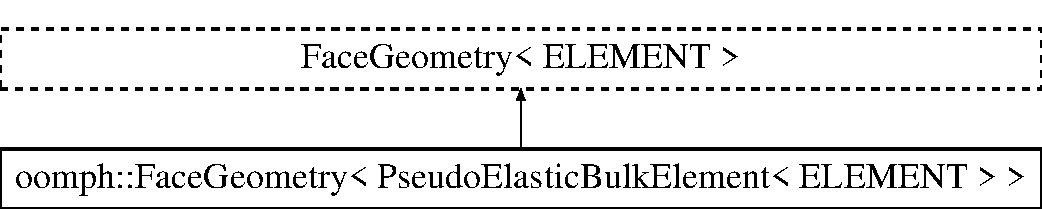
\includegraphics[height=2.000000cm]{classoomph_1_1FaceGeometry_3_01PseudoElasticBulkElement_3_01ELEMENT_01_4_01_4}
\end{center}
\end{figure}
\subsection*{Public Member Functions}
\begin{DoxyCompactItemize}
\item 
\hyperlink{classoomph_1_1FaceGeometry_3_01PseudoElasticBulkElement_3_01ELEMENT_01_4_01_4_a3f79ef40a41543c9d96ef84aecc202f3}{Face\+Geometry} ()
\begin{DoxyCompactList}\small\item\em Constructor -- required for more recent versions of gcc. \end{DoxyCompactList}\end{DoxyCompactItemize}


\subsection{Detailed Description}
\subsubsection*{template$<$class E\+L\+E\+M\+E\+NT$>$\newline
class oomph\+::\+Face\+Geometry$<$ Pseudo\+Elastic\+Bulk\+Element$<$ E\+L\+E\+M\+E\+N\+T $>$ $>$}

Face\+Geometry of wrapped element is the same as the underlying element. 

Definition at line 145 of file prescribed\+\_\+displ\+\_\+lagr\+\_\+mult\+\_\+precond.\+cc.



\subsection{Constructor \& Destructor Documentation}
\mbox{\Hypertarget{classoomph_1_1FaceGeometry_3_01PseudoElasticBulkElement_3_01ELEMENT_01_4_01_4_a3f79ef40a41543c9d96ef84aecc202f3}\label{classoomph_1_1FaceGeometry_3_01PseudoElasticBulkElement_3_01ELEMENT_01_4_01_4_a3f79ef40a41543c9d96ef84aecc202f3}} 
\index{oomph\+::\+Face\+Geometry$<$ Pseudo\+Elastic\+Bulk\+Element$<$ E\+L\+E\+M\+E\+N\+T $>$ $>$@{oomph\+::\+Face\+Geometry$<$ Pseudo\+Elastic\+Bulk\+Element$<$ E\+L\+E\+M\+E\+N\+T $>$ $>$}!Face\+Geometry@{Face\+Geometry}}
\index{Face\+Geometry@{Face\+Geometry}!oomph\+::\+Face\+Geometry$<$ Pseudo\+Elastic\+Bulk\+Element$<$ E\+L\+E\+M\+E\+N\+T $>$ $>$@{oomph\+::\+Face\+Geometry$<$ Pseudo\+Elastic\+Bulk\+Element$<$ E\+L\+E\+M\+E\+N\+T $>$ $>$}}
\subsubsection{\texorpdfstring{Face\+Geometry()}{FaceGeometry()}}
{\footnotesize\ttfamily template$<$class E\+L\+E\+M\+E\+NT $>$ \\
oomph\+::\+Face\+Geometry$<$ \hyperlink{classoomph_1_1PseudoElasticBulkElement}{Pseudo\+Elastic\+Bulk\+Element}$<$ E\+L\+E\+M\+E\+NT $>$ $>$\+::Face\+Geometry (\begin{DoxyParamCaption}{ }\end{DoxyParamCaption})\hspace{0.3cm}{\ttfamily [inline]}}



Constructor -- required for more recent versions of gcc. 



Definition at line 152 of file prescribed\+\_\+displ\+\_\+lagr\+\_\+mult\+\_\+precond.\+cc.



The documentation for this class was generated from the following file\+:\begin{DoxyCompactItemize}
\item 
\hyperlink{prescribed__displ__lagr__mult__precond_8cc}{prescribed\+\_\+displ\+\_\+lagr\+\_\+mult\+\_\+precond.\+cc}\end{DoxyCompactItemize}

\hypertarget{classFSIChannelWithLeafletProblem}{}\section{F\+S\+I\+Channel\+With\+Leaflet\+Problem$<$ E\+L\+E\+M\+E\+NT $>$ Class Template Reference}
\label{classFSIChannelWithLeafletProblem}\index{F\+S\+I\+Channel\+With\+Leaflet\+Problem$<$ E\+L\+E\+M\+E\+N\+T $>$@{F\+S\+I\+Channel\+With\+Leaflet\+Problem$<$ E\+L\+E\+M\+E\+N\+T $>$}}
Inheritance diagram for F\+S\+I\+Channel\+With\+Leaflet\+Problem$<$ E\+L\+E\+M\+E\+NT $>$\+:\begin{figure}[H]
\begin{center}
\leavevmode
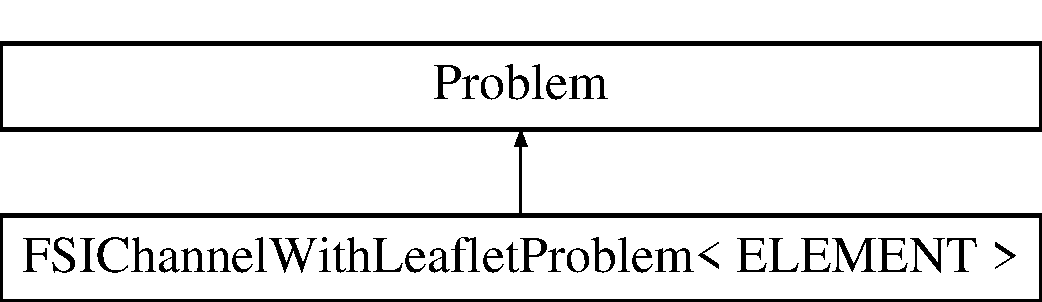
\includegraphics[height=2.000000cm]{classFSIChannelWithLeafletProblem}
\end{center}
\end{figure}
\subsection*{Public Member Functions}
\begin{DoxyCompactItemize}
\item 
\hyperlink{classFSIChannelWithLeafletProblem_a886599acf388d3ad5a2ec8c418c77280}{F\+S\+I\+Channel\+With\+Leaflet\+Problem} (const unsigned \&mesh\+\_\+multiplier)
\begin{DoxyCompactList}\small\item\em Constructor\+: Pass multiplier for uniform mesh refinement. \end{DoxyCompactList}\item 
\hyperlink{classFSIChannelWithLeafletProblem_a5df1d8f7229314a92ffb48ec61f56fe0}{$\sim$\+F\+S\+I\+Channel\+With\+Leaflet\+Problem} ()
\begin{DoxyCompactList}\small\item\em Destructor empty. \end{DoxyCompactList}\item 
void \hyperlink{classFSIChannelWithLeafletProblem_abff6e46a940263c9255a61f649bb4239}{actions\+\_\+after\+\_\+newton\+\_\+solve} ()
\begin{DoxyCompactList}\small\item\em Actions after solve (empty) \end{DoxyCompactList}\item 
void \hyperlink{classFSIChannelWithLeafletProblem_a8a32ef77f32b3283b4b509669deb0a11}{actions\+\_\+before\+\_\+newton\+\_\+solve} ()
\begin{DoxyCompactList}\small\item\em Actions before Newton solve\+: Reset the pseudo-\/elastic undeformed configuration. \end{DoxyCompactList}\item 
void \hyperlink{classFSIChannelWithLeafletProblem_aff02228eddae18ef3d57306ba1e61495}{actions\+\_\+before\+\_\+newton\+\_\+convergence\+\_\+check} ()
\begin{DoxyCompactList}\small\item\em Update no slip before Newton convergence check. \end{DoxyCompactList}\item 
void \hyperlink{classFSIChannelWithLeafletProblem_ac73220fa534cf2409bb0ebcf2fb5e1d5}{actions\+\_\+before\+\_\+implicit\+\_\+timestep} ()
\begin{DoxyCompactList}\small\item\em Actions before implicit timestep\+: Update the inflow velocity. \end{DoxyCompactList}\item 
void \hyperlink{classFSIChannelWithLeafletProblem_a8ca939c0edc4194e4e5cb7d1404f27de}{set\+\_\+iterative\+\_\+solver} ()
\begin{DoxyCompactList}\small\item\em Set iterative solver. \end{DoxyCompactList}\item 
void \hyperlink{classFSIChannelWithLeafletProblem_adca46cd909199b5721b6e17c15caae02}{doc\+\_\+solution} (Doc\+Info \&doc\+\_\+info)
\begin{DoxyCompactList}\small\item\em Doc the solution. \end{DoxyCompactList}\item 
void \hyperlink{classFSIChannelWithLeafletProblem_aa21f42ff019a517d94dbefdfc270c562}{create\+\_\+lagrange\+\_\+multiplier\+\_\+elements} ()
\begin{DoxyCompactList}\small\item\em Create elements that enforce prescribed boundary motion by Lagrange multipliers. \end{DoxyCompactList}\item 
void \hyperlink{classFSIChannelWithLeafletProblem_aeab2d2d99741e64d83792003db758c38}{delete\+\_\+lagrange\+\_\+multiplier\+\_\+elements} ()
\item 
void \hyperlink{classFSIChannelWithLeafletProblem_a27548bcf25ba14dca9f80ffcbc5792b0}{doc\+\_\+parameters} ()
\begin{DoxyCompactList}\small\item\em Doc parameters. \end{DoxyCompactList}\end{DoxyCompactItemize}
\subsection*{Private Member Functions}
\begin{DoxyCompactItemize}
\item 
Node $\ast$ \hyperlink{classFSIChannelWithLeafletProblem_a00605fef274ac93454d59b525ba4d923}{tip\+\_\+node\+\_\+pt} ()
\begin{DoxyCompactList}\small\item\em Helper fct; returns the node at the tip of the wall mesh. \end{DoxyCompactList}\end{DoxyCompactItemize}
\subsection*{Private Attributes}
\begin{DoxyCompactItemize}
\item 
Pseudo\+Elastic\+Channel\+With\+Leaflet\+Mesh$<$ E\+L\+E\+M\+E\+NT $>$ $\ast$ \hyperlink{classFSIChannelWithLeafletProblem_a336bdec3a8b90ac09feb89e5bb3539e8}{Bulk\+\_\+mesh\+\_\+pt}
\begin{DoxyCompactList}\small\item\em Pointer to the fluid mesh. \end{DoxyCompactList}\item 
One\+D\+Lagrangian\+Mesh$<$ F\+S\+I\+Hermite\+Beam\+Element $>$ $\ast$ \hyperlink{classFSIChannelWithLeafletProblem_a943437726f0a54fa8f7fc9ffb12bc4cd}{Wall\+\_\+mesh\+\_\+pt}
\begin{DoxyCompactList}\small\item\em Pointer to the \char`\"{}wall\char`\"{} mesh. \end{DoxyCompactList}\item 
B\+DF$<$ 2 $>$ $\ast$ \hyperlink{classFSIChannelWithLeafletProblem_ac58840d4c2fefae931eb55358099c28d}{Bulk\+\_\+time\+\_\+stepper\+\_\+pt}
\begin{DoxyCompactList}\small\item\em Bulk timestepper. \end{DoxyCompactList}\item 
Newmark$<$ 2 $>$ $\ast$ \hyperlink{classFSIChannelWithLeafletProblem_ace55d5753b8a32fcac448b8a45690afb}{Wall\+\_\+time\+\_\+stepper\+\_\+pt}
\begin{DoxyCompactList}\small\item\em Wall time stepper pt. \end{DoxyCompactList}\item 
Solid\+Mesh $\ast$ \hyperlink{classFSIChannelWithLeafletProblem_aab28704c88d14a2f0975ffcdfbe913e4}{Lagrange\+\_\+multiplier\+\_\+mesh\+\_\+pt}
\begin{DoxyCompactList}\small\item\em Pointers to mesh of Lagrange multiplier elements. \end{DoxyCompactList}\item 
Constitutive\+Law $\ast$ \hyperlink{classFSIChannelWithLeafletProblem_a745553864433ae6c0f1971776249193a}{Constitutive\+\_\+law\+\_\+pt}
\begin{DoxyCompactList}\small\item\em Constitutive law used to determine the mesh deformation. \end{DoxyCompactList}\item 
Mesh\+As\+Geom\+Object $\ast$ \hyperlink{classFSIChannelWithLeafletProblem_a2c6f28af7e78288f5b6d60f69036c8ee}{Wall\+\_\+geom\+\_\+object\+\_\+pt}
\begin{DoxyCompactList}\small\item\em Geometric object for the leaflet (to apply lagrange mult) \end{DoxyCompactList}\item 
\hyperlink{classUndeformedLeaflet}{Undeformed\+Leaflet} $\ast$ \hyperlink{classFSIChannelWithLeafletProblem_adb1d2ebc1379fac8b99cc61379d2b211}{Undeformed\+\_\+wall\+\_\+pt}
\begin{DoxyCompactList}\small\item\em Geom object for the leaflet. \end{DoxyCompactList}\end{DoxyCompactItemize}


\subsection{Detailed Description}
\subsubsection*{template$<$class E\+L\+E\+M\+E\+NT$>$\newline
class F\+S\+I\+Channel\+With\+Leaflet\+Problem$<$ E\+L\+E\+M\+E\+N\+T $>$}

F\+SI leaflet in channel. Mesh update with pseudo-\/elasticity and solved with pseudo-\/elastic fsi preconditioner. 

Definition at line 351 of file fsi\+\_\+channel\+\_\+with\+\_\+leaflet\+\_\+precond.\+cc.



\subsection{Constructor \& Destructor Documentation}
\mbox{\Hypertarget{classFSIChannelWithLeafletProblem_a886599acf388d3ad5a2ec8c418c77280}\label{classFSIChannelWithLeafletProblem_a886599acf388d3ad5a2ec8c418c77280}} 
\index{F\+S\+I\+Channel\+With\+Leaflet\+Problem@{F\+S\+I\+Channel\+With\+Leaflet\+Problem}!F\+S\+I\+Channel\+With\+Leaflet\+Problem@{F\+S\+I\+Channel\+With\+Leaflet\+Problem}}
\index{F\+S\+I\+Channel\+With\+Leaflet\+Problem@{F\+S\+I\+Channel\+With\+Leaflet\+Problem}!F\+S\+I\+Channel\+With\+Leaflet\+Problem@{F\+S\+I\+Channel\+With\+Leaflet\+Problem}}
\subsubsection{\texorpdfstring{F\+S\+I\+Channel\+With\+Leaflet\+Problem()}{FSIChannelWithLeafletProblem()}}
{\footnotesize\ttfamily template$<$class E\+L\+E\+M\+E\+NT $>$ \\
\hyperlink{classFSIChannelWithLeafletProblem}{F\+S\+I\+Channel\+With\+Leaflet\+Problem}$<$ E\+L\+E\+M\+E\+NT $>$\+::\hyperlink{classFSIChannelWithLeafletProblem}{F\+S\+I\+Channel\+With\+Leaflet\+Problem} (\begin{DoxyParamCaption}\item[{const unsigned \&}]{mesh\+\_\+multiplier }\end{DoxyParamCaption})}



Constructor\+: Pass multiplier for uniform mesh refinement. 

Constructor. 

Definition at line 494 of file fsi\+\_\+channel\+\_\+with\+\_\+leaflet\+\_\+precond.\+cc.



References Global\+\_\+\+Parameters\+::\+Fluid\+\_\+height, Global\+\_\+\+Parameters\+::\+Fluid\+\_\+length\+\_\+left, Global\+\_\+\+Parameters\+::\+Fluid\+\_\+length\+\_\+right, Global\+\_\+\+Parameters\+::H, Global\+\_\+\+Parameters\+::\+Lambda\+\_\+sq, Global\+\_\+\+Parameters\+::\+Lambda\+\_\+sq\+\_\+beam, Global\+\_\+\+Parameters\+::\+Leaflet\+\_\+height, Global\+\_\+\+Parameters\+::\+Leaflet\+\_\+x0, Global\+\_\+\+Parameters\+::\+Mesh\+\_\+nleft, Global\+\_\+\+Parameters\+::\+Mesh\+\_\+nright, Global\+\_\+\+Parameters\+::\+Mesh\+\_\+ny1, Global\+\_\+\+Parameters\+::\+Mesh\+\_\+ny2, Global\+\_\+\+Parameters\+::\+Nu, Global\+\_\+\+Parameters\+::Q, Global\+\_\+\+Parameters\+::\+Re, and Global\+\_\+\+Parameters\+::\+Re\+St.

\mbox{\Hypertarget{classFSIChannelWithLeafletProblem_a5df1d8f7229314a92ffb48ec61f56fe0}\label{classFSIChannelWithLeafletProblem_a5df1d8f7229314a92ffb48ec61f56fe0}} 
\index{F\+S\+I\+Channel\+With\+Leaflet\+Problem@{F\+S\+I\+Channel\+With\+Leaflet\+Problem}!````~F\+S\+I\+Channel\+With\+Leaflet\+Problem@{$\sim$\+F\+S\+I\+Channel\+With\+Leaflet\+Problem}}
\index{````~F\+S\+I\+Channel\+With\+Leaflet\+Problem@{$\sim$\+F\+S\+I\+Channel\+With\+Leaflet\+Problem}!F\+S\+I\+Channel\+With\+Leaflet\+Problem@{F\+S\+I\+Channel\+With\+Leaflet\+Problem}}
\subsubsection{\texorpdfstring{$\sim$\+F\+S\+I\+Channel\+With\+Leaflet\+Problem()}{~FSIChannelWithLeafletProblem()}}
{\footnotesize\ttfamily template$<$class E\+L\+E\+M\+E\+NT $>$ \\
\hyperlink{classFSIChannelWithLeafletProblem}{F\+S\+I\+Channel\+With\+Leaflet\+Problem}$<$ E\+L\+E\+M\+E\+NT $>$\+::$\sim$\hyperlink{classFSIChannelWithLeafletProblem}{F\+S\+I\+Channel\+With\+Leaflet\+Problem} (\begin{DoxyParamCaption}{ }\end{DoxyParamCaption})\hspace{0.3cm}{\ttfamily [inline]}}



Destructor empty. 



Definition at line 360 of file fsi\+\_\+channel\+\_\+with\+\_\+leaflet\+\_\+precond.\+cc.



\subsection{Member Function Documentation}
\mbox{\Hypertarget{classFSIChannelWithLeafletProblem_abff6e46a940263c9255a61f649bb4239}\label{classFSIChannelWithLeafletProblem_abff6e46a940263c9255a61f649bb4239}} 
\index{F\+S\+I\+Channel\+With\+Leaflet\+Problem@{F\+S\+I\+Channel\+With\+Leaflet\+Problem}!actions\+\_\+after\+\_\+newton\+\_\+solve@{actions\+\_\+after\+\_\+newton\+\_\+solve}}
\index{actions\+\_\+after\+\_\+newton\+\_\+solve@{actions\+\_\+after\+\_\+newton\+\_\+solve}!F\+S\+I\+Channel\+With\+Leaflet\+Problem@{F\+S\+I\+Channel\+With\+Leaflet\+Problem}}
\subsubsection{\texorpdfstring{actions\+\_\+after\+\_\+newton\+\_\+solve()}{actions\_after\_newton\_solve()}}
{\footnotesize\ttfamily template$<$class E\+L\+E\+M\+E\+NT $>$ \\
void \hyperlink{classFSIChannelWithLeafletProblem}{F\+S\+I\+Channel\+With\+Leaflet\+Problem}$<$ E\+L\+E\+M\+E\+NT $>$\+::actions\+\_\+after\+\_\+newton\+\_\+solve (\begin{DoxyParamCaption}{ }\end{DoxyParamCaption})\hspace{0.3cm}{\ttfamily [inline]}}



Actions after solve (empty) 



Definition at line 373 of file fsi\+\_\+channel\+\_\+with\+\_\+leaflet\+\_\+precond.\+cc.

\mbox{\Hypertarget{classFSIChannelWithLeafletProblem_ac73220fa534cf2409bb0ebcf2fb5e1d5}\label{classFSIChannelWithLeafletProblem_ac73220fa534cf2409bb0ebcf2fb5e1d5}} 
\index{F\+S\+I\+Channel\+With\+Leaflet\+Problem@{F\+S\+I\+Channel\+With\+Leaflet\+Problem}!actions\+\_\+before\+\_\+implicit\+\_\+timestep@{actions\+\_\+before\+\_\+implicit\+\_\+timestep}}
\index{actions\+\_\+before\+\_\+implicit\+\_\+timestep@{actions\+\_\+before\+\_\+implicit\+\_\+timestep}!F\+S\+I\+Channel\+With\+Leaflet\+Problem@{F\+S\+I\+Channel\+With\+Leaflet\+Problem}}
\subsubsection{\texorpdfstring{actions\+\_\+before\+\_\+implicit\+\_\+timestep()}{actions\_before\_implicit\_timestep()}}
{\footnotesize\ttfamily template$<$class E\+L\+E\+M\+E\+NT $>$ \\
void \hyperlink{classFSIChannelWithLeafletProblem}{F\+S\+I\+Channel\+With\+Leaflet\+Problem}$<$ E\+L\+E\+M\+E\+NT $>$\+::actions\+\_\+before\+\_\+implicit\+\_\+timestep (\begin{DoxyParamCaption}{ }\end{DoxyParamCaption})\hspace{0.3cm}{\ttfamily [inline]}}



Actions before implicit timestep\+: Update the inflow velocity. 



Definition at line 396 of file fsi\+\_\+channel\+\_\+with\+\_\+leaflet\+\_\+precond.\+cc.



References Global\+\_\+\+Parameters\+::\+Fluid\+\_\+height, and Global\+\_\+\+Parameters\+::flux().

\mbox{\Hypertarget{classFSIChannelWithLeafletProblem_aff02228eddae18ef3d57306ba1e61495}\label{classFSIChannelWithLeafletProblem_aff02228eddae18ef3d57306ba1e61495}} 
\index{F\+S\+I\+Channel\+With\+Leaflet\+Problem@{F\+S\+I\+Channel\+With\+Leaflet\+Problem}!actions\+\_\+before\+\_\+newton\+\_\+convergence\+\_\+check@{actions\+\_\+before\+\_\+newton\+\_\+convergence\+\_\+check}}
\index{actions\+\_\+before\+\_\+newton\+\_\+convergence\+\_\+check@{actions\+\_\+before\+\_\+newton\+\_\+convergence\+\_\+check}!F\+S\+I\+Channel\+With\+Leaflet\+Problem@{F\+S\+I\+Channel\+With\+Leaflet\+Problem}}
\subsubsection{\texorpdfstring{actions\+\_\+before\+\_\+newton\+\_\+convergence\+\_\+check()}{actions\_before\_newton\_convergence\_check()}}
{\footnotesize\ttfamily template$<$class E\+L\+E\+M\+E\+NT $>$ \\
void \hyperlink{classFSIChannelWithLeafletProblem}{F\+S\+I\+Channel\+With\+Leaflet\+Problem}$<$ E\+L\+E\+M\+E\+NT $>$\+::actions\+\_\+before\+\_\+newton\+\_\+convergence\+\_\+check (\begin{DoxyParamCaption}{ }\end{DoxyParamCaption})\hspace{0.3cm}{\ttfamily [inline]}}



Update no slip before Newton convergence check. 



Definition at line 384 of file fsi\+\_\+channel\+\_\+with\+\_\+leaflet\+\_\+precond.\+cc.

\mbox{\Hypertarget{classFSIChannelWithLeafletProblem_a8a32ef77f32b3283b4b509669deb0a11}\label{classFSIChannelWithLeafletProblem_a8a32ef77f32b3283b4b509669deb0a11}} 
\index{F\+S\+I\+Channel\+With\+Leaflet\+Problem@{F\+S\+I\+Channel\+With\+Leaflet\+Problem}!actions\+\_\+before\+\_\+newton\+\_\+solve@{actions\+\_\+before\+\_\+newton\+\_\+solve}}
\index{actions\+\_\+before\+\_\+newton\+\_\+solve@{actions\+\_\+before\+\_\+newton\+\_\+solve}!F\+S\+I\+Channel\+With\+Leaflet\+Problem@{F\+S\+I\+Channel\+With\+Leaflet\+Problem}}
\subsubsection{\texorpdfstring{actions\+\_\+before\+\_\+newton\+\_\+solve()}{actions\_before\_newton\_solve()}}
{\footnotesize\ttfamily template$<$class E\+L\+E\+M\+E\+NT $>$ \\
void \hyperlink{classFSIChannelWithLeafletProblem}{F\+S\+I\+Channel\+With\+Leaflet\+Problem}$<$ E\+L\+E\+M\+E\+NT $>$\+::actions\+\_\+before\+\_\+newton\+\_\+solve (\begin{DoxyParamCaption}{ }\end{DoxyParamCaption})\hspace{0.3cm}{\ttfamily [inline]}}



Actions before Newton solve\+: Reset the pseudo-\/elastic undeformed configuration. 



Definition at line 377 of file fsi\+\_\+channel\+\_\+with\+\_\+leaflet\+\_\+precond.\+cc.

\mbox{\Hypertarget{classFSIChannelWithLeafletProblem_aa21f42ff019a517d94dbefdfc270c562}\label{classFSIChannelWithLeafletProblem_aa21f42ff019a517d94dbefdfc270c562}} 
\index{F\+S\+I\+Channel\+With\+Leaflet\+Problem@{F\+S\+I\+Channel\+With\+Leaflet\+Problem}!create\+\_\+lagrange\+\_\+multiplier\+\_\+elements@{create\+\_\+lagrange\+\_\+multiplier\+\_\+elements}}
\index{create\+\_\+lagrange\+\_\+multiplier\+\_\+elements@{create\+\_\+lagrange\+\_\+multiplier\+\_\+elements}!F\+S\+I\+Channel\+With\+Leaflet\+Problem@{F\+S\+I\+Channel\+With\+Leaflet\+Problem}}
\subsubsection{\texorpdfstring{create\+\_\+lagrange\+\_\+multiplier\+\_\+elements()}{create\_lagrange\_multiplier\_elements()}}
{\footnotesize\ttfamily template$<$class E\+L\+E\+M\+E\+NT $>$ \\
void \hyperlink{classFSIChannelWithLeafletProblem}{F\+S\+I\+Channel\+With\+Leaflet\+Problem}$<$ E\+L\+E\+M\+E\+NT $>$\+::create\+\_\+lagrange\+\_\+multiplier\+\_\+elements (\begin{DoxyParamCaption}{ }\end{DoxyParamCaption})}



Create elements that enforce prescribed boundary motion by Lagrange multipliers. 

Create elements that impose the prescribed boundary displacement by Lagrange multipliers 

Definition at line 872 of file fsi\+\_\+channel\+\_\+with\+\_\+leaflet\+\_\+precond.\+cc.



References F\+S\+I\+Channel\+With\+Leaflet\+Problem$<$ E\+L\+E\+M\+E\+N\+T $>$\+::delete\+\_\+lagrange\+\_\+multiplier\+\_\+elements().



Referenced by F\+S\+I\+Channel\+With\+Leaflet\+Problem$<$ E\+L\+E\+M\+E\+N\+T $>$\+::set\+\_\+iterative\+\_\+solver().

\mbox{\Hypertarget{classFSIChannelWithLeafletProblem_aeab2d2d99741e64d83792003db758c38}\label{classFSIChannelWithLeafletProblem_aeab2d2d99741e64d83792003db758c38}} 
\index{F\+S\+I\+Channel\+With\+Leaflet\+Problem@{F\+S\+I\+Channel\+With\+Leaflet\+Problem}!delete\+\_\+lagrange\+\_\+multiplier\+\_\+elements@{delete\+\_\+lagrange\+\_\+multiplier\+\_\+elements}}
\index{delete\+\_\+lagrange\+\_\+multiplier\+\_\+elements@{delete\+\_\+lagrange\+\_\+multiplier\+\_\+elements}!F\+S\+I\+Channel\+With\+Leaflet\+Problem@{F\+S\+I\+Channel\+With\+Leaflet\+Problem}}
\subsubsection{\texorpdfstring{delete\+\_\+lagrange\+\_\+multiplier\+\_\+elements()}{delete\_lagrange\_multiplier\_elements()}}
{\footnotesize\ttfamily template$<$class E\+L\+E\+M\+E\+NT $>$ \\
void \hyperlink{classFSIChannelWithLeafletProblem}{F\+S\+I\+Channel\+With\+Leaflet\+Problem}$<$ E\+L\+E\+M\+E\+NT $>$\+::delete\+\_\+lagrange\+\_\+multiplier\+\_\+elements (\begin{DoxyParamCaption}{ }\end{DoxyParamCaption})}

Delete elements that enforce prescribed boundary motion by Lagrange multipliers

Delete elements that impose the prescribed boundary displacement and wipe the associated mesh 

Definition at line 947 of file fsi\+\_\+channel\+\_\+with\+\_\+leaflet\+\_\+precond.\+cc.



Referenced by F\+S\+I\+Channel\+With\+Leaflet\+Problem$<$ E\+L\+E\+M\+E\+N\+T $>$\+::create\+\_\+lagrange\+\_\+multiplier\+\_\+elements().

\mbox{\Hypertarget{classFSIChannelWithLeafletProblem_a27548bcf25ba14dca9f80ffcbc5792b0}\label{classFSIChannelWithLeafletProblem_a27548bcf25ba14dca9f80ffcbc5792b0}} 
\index{F\+S\+I\+Channel\+With\+Leaflet\+Problem@{F\+S\+I\+Channel\+With\+Leaflet\+Problem}!doc\+\_\+parameters@{doc\+\_\+parameters}}
\index{doc\+\_\+parameters@{doc\+\_\+parameters}!F\+S\+I\+Channel\+With\+Leaflet\+Problem@{F\+S\+I\+Channel\+With\+Leaflet\+Problem}}
\subsubsection{\texorpdfstring{doc\+\_\+parameters()}{doc\_parameters()}}
{\footnotesize\ttfamily template$<$class E\+L\+E\+M\+E\+NT $>$ \\
void \hyperlink{classFSIChannelWithLeafletProblem}{F\+S\+I\+Channel\+With\+Leaflet\+Problem}$<$ E\+L\+E\+M\+E\+NT $>$\+::doc\+\_\+parameters (\begin{DoxyParamCaption}{ }\end{DoxyParamCaption})\hspace{0.3cm}{\ttfamily [inline]}}



Doc parameters. 



Definition at line 432 of file fsi\+\_\+channel\+\_\+with\+\_\+leaflet\+\_\+precond.\+cc.



References Global\+\_\+\+Parameters\+::\+Lambda\+\_\+sq\+\_\+beam, Global\+\_\+\+Parameters\+::Q, Global\+\_\+\+Parameters\+::\+Re, and Global\+\_\+\+Parameters\+::T.

\mbox{\Hypertarget{classFSIChannelWithLeafletProblem_adca46cd909199b5721b6e17c15caae02}\label{classFSIChannelWithLeafletProblem_adca46cd909199b5721b6e17c15caae02}} 
\index{F\+S\+I\+Channel\+With\+Leaflet\+Problem@{F\+S\+I\+Channel\+With\+Leaflet\+Problem}!doc\+\_\+solution@{doc\+\_\+solution}}
\index{doc\+\_\+solution@{doc\+\_\+solution}!F\+S\+I\+Channel\+With\+Leaflet\+Problem@{F\+S\+I\+Channel\+With\+Leaflet\+Problem}}
\subsubsection{\texorpdfstring{doc\+\_\+solution()}{doc\_solution()}}
{\footnotesize\ttfamily template$<$class E\+L\+E\+M\+E\+NT $>$ \\
void \hyperlink{classFSIChannelWithLeafletProblem}{F\+S\+I\+Channel\+With\+Leaflet\+Problem}$<$ E\+L\+E\+M\+E\+NT $>$\+::doc\+\_\+solution (\begin{DoxyParamCaption}\item[{Doc\+Info \&}]{doc\+\_\+info }\end{DoxyParamCaption})}



Doc the solution. 



Definition at line 970 of file fsi\+\_\+channel\+\_\+with\+\_\+leaflet\+\_\+precond.\+cc.

\mbox{\Hypertarget{classFSIChannelWithLeafletProblem_a8ca939c0edc4194e4e5cb7d1404f27de}\label{classFSIChannelWithLeafletProblem_a8ca939c0edc4194e4e5cb7d1404f27de}} 
\index{F\+S\+I\+Channel\+With\+Leaflet\+Problem@{F\+S\+I\+Channel\+With\+Leaflet\+Problem}!set\+\_\+iterative\+\_\+solver@{set\+\_\+iterative\+\_\+solver}}
\index{set\+\_\+iterative\+\_\+solver@{set\+\_\+iterative\+\_\+solver}!F\+S\+I\+Channel\+With\+Leaflet\+Problem@{F\+S\+I\+Channel\+With\+Leaflet\+Problem}}
\subsubsection{\texorpdfstring{set\+\_\+iterative\+\_\+solver()}{set\_iterative\_solver()}}
{\footnotesize\ttfamily template$<$class E\+L\+E\+M\+E\+NT $>$ \\
void \hyperlink{classFSIChannelWithLeafletProblem}{F\+S\+I\+Channel\+With\+Leaflet\+Problem}$<$ E\+L\+E\+M\+E\+NT $>$\+::set\+\_\+iterative\+\_\+solver (\begin{DoxyParamCaption}{ }\end{DoxyParamCaption})}



Set iterative solver. 



Definition at line 737 of file fsi\+\_\+channel\+\_\+with\+\_\+leaflet\+\_\+precond.\+cc.



References F\+S\+I\+Channel\+With\+Leaflet\+Problem$<$ E\+L\+E\+M\+E\+N\+T $>$\+::create\+\_\+lagrange\+\_\+multiplier\+\_\+elements(), and L\+S\+C\+\_\+\+Preconditioner\+\_\+\+Helper\+::set\+\_\+hypre\+\_\+preconditioner().

\mbox{\Hypertarget{classFSIChannelWithLeafletProblem_a00605fef274ac93454d59b525ba4d923}\label{classFSIChannelWithLeafletProblem_a00605fef274ac93454d59b525ba4d923}} 
\index{F\+S\+I\+Channel\+With\+Leaflet\+Problem@{F\+S\+I\+Channel\+With\+Leaflet\+Problem}!tip\+\_\+node\+\_\+pt@{tip\+\_\+node\+\_\+pt}}
\index{tip\+\_\+node\+\_\+pt@{tip\+\_\+node\+\_\+pt}!F\+S\+I\+Channel\+With\+Leaflet\+Problem@{F\+S\+I\+Channel\+With\+Leaflet\+Problem}}
\subsubsection{\texorpdfstring{tip\+\_\+node\+\_\+pt()}{tip\_node\_pt()}}
{\footnotesize\ttfamily template$<$class E\+L\+E\+M\+E\+NT $>$ \\
Node$\ast$ \hyperlink{classFSIChannelWithLeafletProblem}{F\+S\+I\+Channel\+With\+Leaflet\+Problem}$<$ E\+L\+E\+M\+E\+NT $>$\+::tip\+\_\+node\+\_\+pt (\begin{DoxyParamCaption}{ }\end{DoxyParamCaption})\hspace{0.3cm}{\ttfamily [inline]}, {\ttfamily [private]}}



Helper fct; returns the node at the tip of the wall mesh. 



Definition at line 455 of file fsi\+\_\+channel\+\_\+with\+\_\+leaflet\+\_\+precond.\+cc.



\subsection{Member Data Documentation}
\mbox{\Hypertarget{classFSIChannelWithLeafletProblem_a336bdec3a8b90ac09feb89e5bb3539e8}\label{classFSIChannelWithLeafletProblem_a336bdec3a8b90ac09feb89e5bb3539e8}} 
\index{F\+S\+I\+Channel\+With\+Leaflet\+Problem@{F\+S\+I\+Channel\+With\+Leaflet\+Problem}!Bulk\+\_\+mesh\+\_\+pt@{Bulk\+\_\+mesh\+\_\+pt}}
\index{Bulk\+\_\+mesh\+\_\+pt@{Bulk\+\_\+mesh\+\_\+pt}!F\+S\+I\+Channel\+With\+Leaflet\+Problem@{F\+S\+I\+Channel\+With\+Leaflet\+Problem}}
\subsubsection{\texorpdfstring{Bulk\+\_\+mesh\+\_\+pt}{Bulk\_mesh\_pt}}
{\footnotesize\ttfamily template$<$class E\+L\+E\+M\+E\+NT $>$ \\
Pseudo\+Elastic\+Channel\+With\+Leaflet\+Mesh$<$E\+L\+E\+M\+E\+NT$>$$\ast$ \hyperlink{classFSIChannelWithLeafletProblem}{F\+S\+I\+Channel\+With\+Leaflet\+Problem}$<$ E\+L\+E\+M\+E\+NT $>$\+::Bulk\+\_\+mesh\+\_\+pt\hspace{0.3cm}{\ttfamily [private]}}



Pointer to the fluid mesh. 



Definition at line 463 of file fsi\+\_\+channel\+\_\+with\+\_\+leaflet\+\_\+precond.\+cc.

\mbox{\Hypertarget{classFSIChannelWithLeafletProblem_ac58840d4c2fefae931eb55358099c28d}\label{classFSIChannelWithLeafletProblem_ac58840d4c2fefae931eb55358099c28d}} 
\index{F\+S\+I\+Channel\+With\+Leaflet\+Problem@{F\+S\+I\+Channel\+With\+Leaflet\+Problem}!Bulk\+\_\+time\+\_\+stepper\+\_\+pt@{Bulk\+\_\+time\+\_\+stepper\+\_\+pt}}
\index{Bulk\+\_\+time\+\_\+stepper\+\_\+pt@{Bulk\+\_\+time\+\_\+stepper\+\_\+pt}!F\+S\+I\+Channel\+With\+Leaflet\+Problem@{F\+S\+I\+Channel\+With\+Leaflet\+Problem}}
\subsubsection{\texorpdfstring{Bulk\+\_\+time\+\_\+stepper\+\_\+pt}{Bulk\_time\_stepper\_pt}}
{\footnotesize\ttfamily template$<$class E\+L\+E\+M\+E\+NT $>$ \\
B\+DF$<$2$>$$\ast$ \hyperlink{classFSIChannelWithLeafletProblem}{F\+S\+I\+Channel\+With\+Leaflet\+Problem}$<$ E\+L\+E\+M\+E\+NT $>$\+::Bulk\+\_\+time\+\_\+stepper\+\_\+pt\hspace{0.3cm}{\ttfamily [private]}}



Bulk timestepper. 



Definition at line 469 of file fsi\+\_\+channel\+\_\+with\+\_\+leaflet\+\_\+precond.\+cc.

\mbox{\Hypertarget{classFSIChannelWithLeafletProblem_a745553864433ae6c0f1971776249193a}\label{classFSIChannelWithLeafletProblem_a745553864433ae6c0f1971776249193a}} 
\index{F\+S\+I\+Channel\+With\+Leaflet\+Problem@{F\+S\+I\+Channel\+With\+Leaflet\+Problem}!Constitutive\+\_\+law\+\_\+pt@{Constitutive\+\_\+law\+\_\+pt}}
\index{Constitutive\+\_\+law\+\_\+pt@{Constitutive\+\_\+law\+\_\+pt}!F\+S\+I\+Channel\+With\+Leaflet\+Problem@{F\+S\+I\+Channel\+With\+Leaflet\+Problem}}
\subsubsection{\texorpdfstring{Constitutive\+\_\+law\+\_\+pt}{Constitutive\_law\_pt}}
{\footnotesize\ttfamily template$<$class E\+L\+E\+M\+E\+NT $>$ \\
Constitutive\+Law$\ast$ \hyperlink{classFSIChannelWithLeafletProblem}{F\+S\+I\+Channel\+With\+Leaflet\+Problem}$<$ E\+L\+E\+M\+E\+NT $>$\+::Constitutive\+\_\+law\+\_\+pt\hspace{0.3cm}{\ttfamily [private]}}



Constitutive law used to determine the mesh deformation. 



Definition at line 478 of file fsi\+\_\+channel\+\_\+with\+\_\+leaflet\+\_\+precond.\+cc.

\mbox{\Hypertarget{classFSIChannelWithLeafletProblem_aab28704c88d14a2f0975ffcdfbe913e4}\label{classFSIChannelWithLeafletProblem_aab28704c88d14a2f0975ffcdfbe913e4}} 
\index{F\+S\+I\+Channel\+With\+Leaflet\+Problem@{F\+S\+I\+Channel\+With\+Leaflet\+Problem}!Lagrange\+\_\+multiplier\+\_\+mesh\+\_\+pt@{Lagrange\+\_\+multiplier\+\_\+mesh\+\_\+pt}}
\index{Lagrange\+\_\+multiplier\+\_\+mesh\+\_\+pt@{Lagrange\+\_\+multiplier\+\_\+mesh\+\_\+pt}!F\+S\+I\+Channel\+With\+Leaflet\+Problem@{F\+S\+I\+Channel\+With\+Leaflet\+Problem}}
\subsubsection{\texorpdfstring{Lagrange\+\_\+multiplier\+\_\+mesh\+\_\+pt}{Lagrange\_multiplier\_mesh\_pt}}
{\footnotesize\ttfamily template$<$class E\+L\+E\+M\+E\+NT $>$ \\
Solid\+Mesh$\ast$ \hyperlink{classFSIChannelWithLeafletProblem}{F\+S\+I\+Channel\+With\+Leaflet\+Problem}$<$ E\+L\+E\+M\+E\+NT $>$\+::Lagrange\+\_\+multiplier\+\_\+mesh\+\_\+pt\hspace{0.3cm}{\ttfamily [private]}}



Pointers to mesh of Lagrange multiplier elements. 



Definition at line 475 of file fsi\+\_\+channel\+\_\+with\+\_\+leaflet\+\_\+precond.\+cc.

\mbox{\Hypertarget{classFSIChannelWithLeafletProblem_adb1d2ebc1379fac8b99cc61379d2b211}\label{classFSIChannelWithLeafletProblem_adb1d2ebc1379fac8b99cc61379d2b211}} 
\index{F\+S\+I\+Channel\+With\+Leaflet\+Problem@{F\+S\+I\+Channel\+With\+Leaflet\+Problem}!Undeformed\+\_\+wall\+\_\+pt@{Undeformed\+\_\+wall\+\_\+pt}}
\index{Undeformed\+\_\+wall\+\_\+pt@{Undeformed\+\_\+wall\+\_\+pt}!F\+S\+I\+Channel\+With\+Leaflet\+Problem@{F\+S\+I\+Channel\+With\+Leaflet\+Problem}}
\subsubsection{\texorpdfstring{Undeformed\+\_\+wall\+\_\+pt}{Undeformed\_wall\_pt}}
{\footnotesize\ttfamily template$<$class E\+L\+E\+M\+E\+NT $>$ \\
\hyperlink{classUndeformedLeaflet}{Undeformed\+Leaflet}$\ast$ \hyperlink{classFSIChannelWithLeafletProblem}{F\+S\+I\+Channel\+With\+Leaflet\+Problem}$<$ E\+L\+E\+M\+E\+NT $>$\+::Undeformed\+\_\+wall\+\_\+pt\hspace{0.3cm}{\ttfamily [private]}}



Geom object for the leaflet. 



Definition at line 484 of file fsi\+\_\+channel\+\_\+with\+\_\+leaflet\+\_\+precond.\+cc.

\mbox{\Hypertarget{classFSIChannelWithLeafletProblem_a2c6f28af7e78288f5b6d60f69036c8ee}\label{classFSIChannelWithLeafletProblem_a2c6f28af7e78288f5b6d60f69036c8ee}} 
\index{F\+S\+I\+Channel\+With\+Leaflet\+Problem@{F\+S\+I\+Channel\+With\+Leaflet\+Problem}!Wall\+\_\+geom\+\_\+object\+\_\+pt@{Wall\+\_\+geom\+\_\+object\+\_\+pt}}
\index{Wall\+\_\+geom\+\_\+object\+\_\+pt@{Wall\+\_\+geom\+\_\+object\+\_\+pt}!F\+S\+I\+Channel\+With\+Leaflet\+Problem@{F\+S\+I\+Channel\+With\+Leaflet\+Problem}}
\subsubsection{\texorpdfstring{Wall\+\_\+geom\+\_\+object\+\_\+pt}{Wall\_geom\_object\_pt}}
{\footnotesize\ttfamily template$<$class E\+L\+E\+M\+E\+NT $>$ \\
Mesh\+As\+Geom\+Object$\ast$ \hyperlink{classFSIChannelWithLeafletProblem}{F\+S\+I\+Channel\+With\+Leaflet\+Problem}$<$ E\+L\+E\+M\+E\+NT $>$\+::Wall\+\_\+geom\+\_\+object\+\_\+pt\hspace{0.3cm}{\ttfamily [private]}}



Geometric object for the leaflet (to apply lagrange mult) 



Definition at line 481 of file fsi\+\_\+channel\+\_\+with\+\_\+leaflet\+\_\+precond.\+cc.

\mbox{\Hypertarget{classFSIChannelWithLeafletProblem_a943437726f0a54fa8f7fc9ffb12bc4cd}\label{classFSIChannelWithLeafletProblem_a943437726f0a54fa8f7fc9ffb12bc4cd}} 
\index{F\+S\+I\+Channel\+With\+Leaflet\+Problem@{F\+S\+I\+Channel\+With\+Leaflet\+Problem}!Wall\+\_\+mesh\+\_\+pt@{Wall\+\_\+mesh\+\_\+pt}}
\index{Wall\+\_\+mesh\+\_\+pt@{Wall\+\_\+mesh\+\_\+pt}!F\+S\+I\+Channel\+With\+Leaflet\+Problem@{F\+S\+I\+Channel\+With\+Leaflet\+Problem}}
\subsubsection{\texorpdfstring{Wall\+\_\+mesh\+\_\+pt}{Wall\_mesh\_pt}}
{\footnotesize\ttfamily template$<$class E\+L\+E\+M\+E\+NT $>$ \\
One\+D\+Lagrangian\+Mesh$<$F\+S\+I\+Hermite\+Beam\+Element$>$$\ast$ \hyperlink{classFSIChannelWithLeafletProblem}{F\+S\+I\+Channel\+With\+Leaflet\+Problem}$<$ E\+L\+E\+M\+E\+NT $>$\+::Wall\+\_\+mesh\+\_\+pt\hspace{0.3cm}{\ttfamily [private]}}



Pointer to the \char`\"{}wall\char`\"{} mesh. 



Definition at line 466 of file fsi\+\_\+channel\+\_\+with\+\_\+leaflet\+\_\+precond.\+cc.

\mbox{\Hypertarget{classFSIChannelWithLeafletProblem_ace55d5753b8a32fcac448b8a45690afb}\label{classFSIChannelWithLeafletProblem_ace55d5753b8a32fcac448b8a45690afb}} 
\index{F\+S\+I\+Channel\+With\+Leaflet\+Problem@{F\+S\+I\+Channel\+With\+Leaflet\+Problem}!Wall\+\_\+time\+\_\+stepper\+\_\+pt@{Wall\+\_\+time\+\_\+stepper\+\_\+pt}}
\index{Wall\+\_\+time\+\_\+stepper\+\_\+pt@{Wall\+\_\+time\+\_\+stepper\+\_\+pt}!F\+S\+I\+Channel\+With\+Leaflet\+Problem@{F\+S\+I\+Channel\+With\+Leaflet\+Problem}}
\subsubsection{\texorpdfstring{Wall\+\_\+time\+\_\+stepper\+\_\+pt}{Wall\_time\_stepper\_pt}}
{\footnotesize\ttfamily template$<$class E\+L\+E\+M\+E\+NT $>$ \\
Newmark$<$2$>$$\ast$ \hyperlink{classFSIChannelWithLeafletProblem}{F\+S\+I\+Channel\+With\+Leaflet\+Problem}$<$ E\+L\+E\+M\+E\+NT $>$\+::Wall\+\_\+time\+\_\+stepper\+\_\+pt\hspace{0.3cm}{\ttfamily [private]}}



Wall time stepper pt. 



Definition at line 472 of file fsi\+\_\+channel\+\_\+with\+\_\+leaflet\+\_\+precond.\+cc.



The documentation for this class was generated from the following file\+:\begin{DoxyCompactItemize}
\item 
\hyperlink{fsi__channel__with__leaflet__precond_8cc}{fsi\+\_\+channel\+\_\+with\+\_\+leaflet\+\_\+precond.\+cc}\end{DoxyCompactItemize}

\hypertarget{classoomph_1_1PseudoElasticBulkElement}{}\section{oomph\+:\+:Pseudo\+Elastic\+Bulk\+Element$<$ E\+L\+E\+M\+E\+NT $>$ Class Template Reference}
\label{classoomph_1_1PseudoElasticBulkElement}\index{oomph\+::\+Pseudo\+Elastic\+Bulk\+Element$<$ E\+L\+E\+M\+E\+N\+T $>$@{oomph\+::\+Pseudo\+Elastic\+Bulk\+Element$<$ E\+L\+E\+M\+E\+N\+T $>$}}
Inheritance diagram for oomph\+:\+:Pseudo\+Elastic\+Bulk\+Element$<$ E\+L\+E\+M\+E\+NT $>$\+:\begin{figure}[H]
\begin{center}
\leavevmode
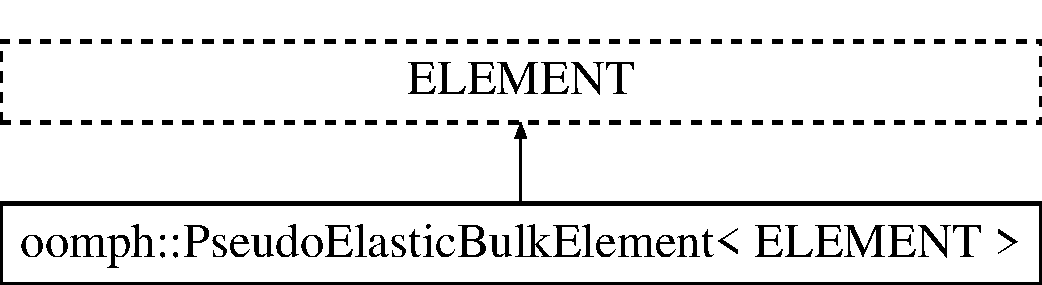
\includegraphics[height=2.000000cm]{classoomph_1_1PseudoElasticBulkElement}
\end{center}
\end{figure}
\subsection*{Public Member Functions}
\begin{DoxyCompactItemize}
\item 
\hyperlink{classoomph_1_1PseudoElasticBulkElement_a38c03edd9639522e713ef9bf679d7e5a}{Pseudo\+Elastic\+Bulk\+Element} ()
\begin{DoxyCompactList}\small\item\em Constructor. \end{DoxyCompactList}\item 
unsigned \hyperlink{classoomph_1_1PseudoElasticBulkElement_a18674d52b96db8800d31e89ffd465175}{ndof\+\_\+types} () const
\begin{DoxyCompactList}\small\item\em Returns the number of D\+OF types associated with this element\+: Twice the number of spatial dimensions (for the constrained and unconstrained nodal positions). \end{DoxyCompactList}\item 
void \hyperlink{classoomph_1_1PseudoElasticBulkElement_a8f1dc2011100324953293470a18f3080}{get\+\_\+dof\+\_\+numbers\+\_\+for\+\_\+unknowns} (std\+::list$<$ std\+::pair$<$ unsigned long, unsigned $>$ $>$ \&dof\+\_\+lookup\+\_\+list) const
\begin{DoxyCompactList}\small\item\em Create a list of pairs for all unknowns in this element, so that the first entry in each pair contains the global equation number of the unknown, while the second one contains the number of the \char`\"{}\+D\+O\+F\char`\"{} that this unknown is associated with. (Function can obviously only be called if the equation numbering scheme has been set up.)~\newline
E.\+g. in a 3D problem there are 6 types of D\+OF\+:~\newline
0 -\/ x displacement (without lagr mult traction)~\newline
1 -\/ y displacement (without lagr mult traction)~\newline
2 -\/ z displacement (without lagr mult traction)~\newline
4 -\/ x displacement (with lagr mult traction)~\newline
5 -\/ y displacement (with lagr mult traction)~\newline
6 -\/ z displacement (with lagr mult traction)~\newline
. \end{DoxyCompactList}\end{DoxyCompactItemize}


\subsection{Detailed Description}
\subsubsection*{template$<$class E\+L\+E\+M\+E\+NT$>$\newline
class oomph\+::\+Pseudo\+Elastic\+Bulk\+Element$<$ E\+L\+E\+M\+E\+N\+T $>$}

Pseudo-\/\+Elastic Solid element class to overload the block preconditioner methods \hyperlink{classoomph_1_1PseudoElasticBulkElement_a18674d52b96db8800d31e89ffd465175}{ndof\+\_\+types()} and \hyperlink{classoomph_1_1PseudoElasticBulkElement_a8f1dc2011100324953293470a18f3080}{get\+\_\+dof\+\_\+numbers\+\_\+for\+\_\+unknowns()} to differentiate between D\+O\+Fs subject to Lagrange multiplier and those that are not. 

Definition at line 58 of file prescribed\+\_\+displ\+\_\+lagr\+\_\+mult\+\_\+precond.\+cc.



\subsection{Constructor \& Destructor Documentation}
\mbox{\Hypertarget{classoomph_1_1PseudoElasticBulkElement_a38c03edd9639522e713ef9bf679d7e5a}\label{classoomph_1_1PseudoElasticBulkElement_a38c03edd9639522e713ef9bf679d7e5a}} 
\index{oomph\+::\+Pseudo\+Elastic\+Bulk\+Element@{oomph\+::\+Pseudo\+Elastic\+Bulk\+Element}!Pseudo\+Elastic\+Bulk\+Element@{Pseudo\+Elastic\+Bulk\+Element}}
\index{Pseudo\+Elastic\+Bulk\+Element@{Pseudo\+Elastic\+Bulk\+Element}!oomph\+::\+Pseudo\+Elastic\+Bulk\+Element@{oomph\+::\+Pseudo\+Elastic\+Bulk\+Element}}
\subsubsection{\texorpdfstring{Pseudo\+Elastic\+Bulk\+Element()}{PseudoElasticBulkElement()}}
{\footnotesize\ttfamily template$<$class E\+L\+E\+M\+E\+NT $>$ \\
\hyperlink{classoomph_1_1PseudoElasticBulkElement}{oomph\+::\+Pseudo\+Elastic\+Bulk\+Element}$<$ E\+L\+E\+M\+E\+NT $>$\+::\hyperlink{classoomph_1_1PseudoElasticBulkElement}{Pseudo\+Elastic\+Bulk\+Element} (\begin{DoxyParamCaption}{ }\end{DoxyParamCaption})\hspace{0.3cm}{\ttfamily [inline]}}



Constructor. 



Definition at line 65 of file prescribed\+\_\+displ\+\_\+lagr\+\_\+mult\+\_\+precond.\+cc.



\subsection{Member Function Documentation}
\mbox{\Hypertarget{classoomph_1_1PseudoElasticBulkElement_a8f1dc2011100324953293470a18f3080}\label{classoomph_1_1PseudoElasticBulkElement_a8f1dc2011100324953293470a18f3080}} 
\index{oomph\+::\+Pseudo\+Elastic\+Bulk\+Element@{oomph\+::\+Pseudo\+Elastic\+Bulk\+Element}!get\+\_\+dof\+\_\+numbers\+\_\+for\+\_\+unknowns@{get\+\_\+dof\+\_\+numbers\+\_\+for\+\_\+unknowns}}
\index{get\+\_\+dof\+\_\+numbers\+\_\+for\+\_\+unknowns@{get\+\_\+dof\+\_\+numbers\+\_\+for\+\_\+unknowns}!oomph\+::\+Pseudo\+Elastic\+Bulk\+Element@{oomph\+::\+Pseudo\+Elastic\+Bulk\+Element}}
\subsubsection{\texorpdfstring{get\+\_\+dof\+\_\+numbers\+\_\+for\+\_\+unknowns()}{get\_dof\_numbers\_for\_unknowns()}}
{\footnotesize\ttfamily template$<$class E\+L\+E\+M\+E\+NT $>$ \\
void \hyperlink{classoomph_1_1PseudoElasticBulkElement}{oomph\+::\+Pseudo\+Elastic\+Bulk\+Element}$<$ E\+L\+E\+M\+E\+NT $>$\+::get\+\_\+dof\+\_\+numbers\+\_\+for\+\_\+unknowns (\begin{DoxyParamCaption}\item[{std\+::list$<$ std\+::pair$<$ unsigned long, unsigned $>$ $>$ \&}]{dof\+\_\+lookup\+\_\+list }\end{DoxyParamCaption}) const\hspace{0.3cm}{\ttfamily [inline]}}



Create a list of pairs for all unknowns in this element, so that the first entry in each pair contains the global equation number of the unknown, while the second one contains the number of the \char`\"{}\+D\+O\+F\char`\"{} that this unknown is associated with. (Function can obviously only be called if the equation numbering scheme has been set up.)~\newline
E.\+g. in a 3D problem there are 6 types of D\+OF\+:~\newline
0 -\/ x displacement (without lagr mult traction)~\newline
1 -\/ y displacement (without lagr mult traction)~\newline
2 -\/ z displacement (without lagr mult traction)~\newline
4 -\/ x displacement (with lagr mult traction)~\newline
5 -\/ y displacement (with lagr mult traction)~\newline
6 -\/ z displacement (with lagr mult traction)~\newline
. 



Definition at line 88 of file prescribed\+\_\+displ\+\_\+lagr\+\_\+mult\+\_\+precond.\+cc.

\mbox{\Hypertarget{classoomph_1_1PseudoElasticBulkElement_a18674d52b96db8800d31e89ffd465175}\label{classoomph_1_1PseudoElasticBulkElement_a18674d52b96db8800d31e89ffd465175}} 
\index{oomph\+::\+Pseudo\+Elastic\+Bulk\+Element@{oomph\+::\+Pseudo\+Elastic\+Bulk\+Element}!ndof\+\_\+types@{ndof\+\_\+types}}
\index{ndof\+\_\+types@{ndof\+\_\+types}!oomph\+::\+Pseudo\+Elastic\+Bulk\+Element@{oomph\+::\+Pseudo\+Elastic\+Bulk\+Element}}
\subsubsection{\texorpdfstring{ndof\+\_\+types()}{ndof\_types()}}
{\footnotesize\ttfamily template$<$class E\+L\+E\+M\+E\+NT $>$ \\
unsigned \hyperlink{classoomph_1_1PseudoElasticBulkElement}{oomph\+::\+Pseudo\+Elastic\+Bulk\+Element}$<$ E\+L\+E\+M\+E\+NT $>$\+::ndof\+\_\+types (\begin{DoxyParamCaption}{ }\end{DoxyParamCaption}) const\hspace{0.3cm}{\ttfamily [inline]}}



Returns the number of D\+OF types associated with this element\+: Twice the number of spatial dimensions (for the constrained and unconstrained nodal positions). 



Definition at line 70 of file prescribed\+\_\+displ\+\_\+lagr\+\_\+mult\+\_\+precond.\+cc.



The documentation for this class was generated from the following file\+:\begin{DoxyCompactItemize}
\item 
\hyperlink{prescribed__displ__lagr__mult__precond_8cc}{prescribed\+\_\+displ\+\_\+lagr\+\_\+mult\+\_\+precond.\+cc}\end{DoxyCompactItemize}

\hypertarget{classUndeformedLeaflet}{}\section{Undeformed\+Leaflet Class Reference}
\label{classUndeformedLeaflet}\index{Undeformed\+Leaflet@{Undeformed\+Leaflet}}


Geom\+Object\+: Undeformed straight, vertical leaflet.  


Inheritance diagram for Undeformed\+Leaflet\+:\begin{figure}[H]
\begin{center}
\leavevmode
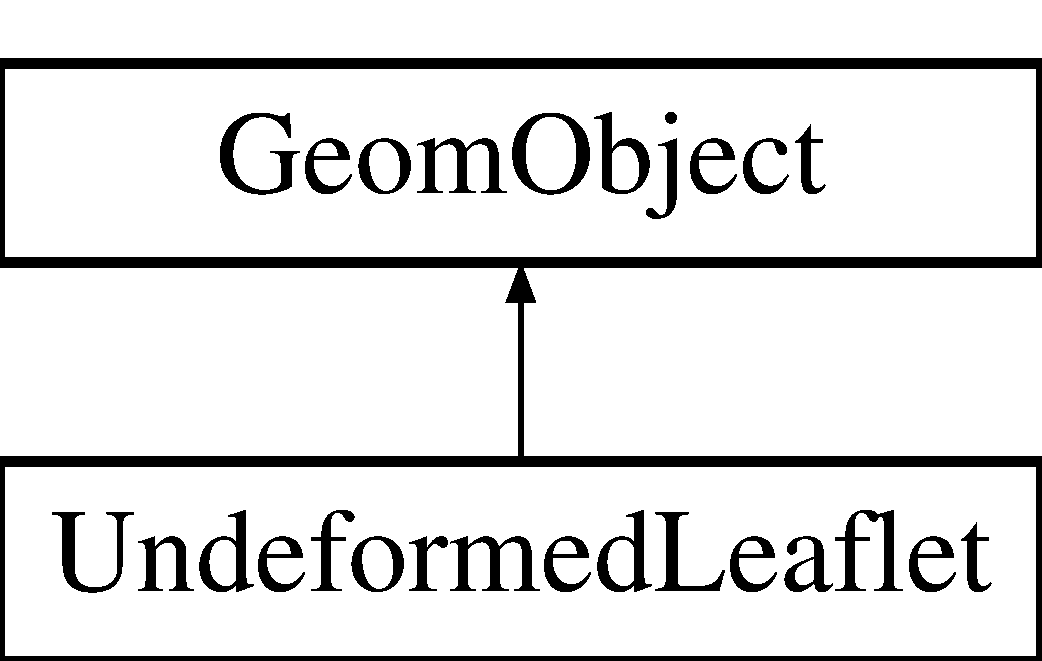
\includegraphics[height=2.000000cm]{classUndeformedLeaflet}
\end{center}
\end{figure}
\subsection*{Public Member Functions}
\begin{DoxyCompactItemize}
\item 
\hyperlink{classUndeformedLeaflet_ac4c0478b1f329360684af14b59043b12}{Undeformed\+Leaflet} (const double \&x0)
\begin{DoxyCompactList}\small\item\em Constructor\+: argument is the x-\/coordinate of the leaflet. \end{DoxyCompactList}\item 
void \hyperlink{classUndeformedLeaflet_a8e9b79702eb9a38e19886b84aeb47918}{position} (const Vector$<$ double $>$ \&zeta, Vector$<$ double $>$ \&r) const
\begin{DoxyCompactList}\small\item\em Position vector at Lagrangian coordinate zeta. \end{DoxyCompactList}\item 
void \hyperlink{classUndeformedLeaflet_a6949784da1030dd63ef741d170ef9798}{position} (const unsigned \&t, const Vector$<$ double $>$ \&zeta, Vector$<$ double $>$ \&r) const
\begin{DoxyCompactList}\small\item\em Parametrised position on object\+: r(zeta). Evaluated at previous timestep. t=0\+: current time; t$>$0\+: previous timestep. Calls steady version. \end{DoxyCompactList}\item 
void \hyperlink{classUndeformedLeaflet_a47d674756ce22e00a44ca0bd030a99da}{d2position} (const Vector$<$ double $>$ \&zeta, Vector$<$ double $>$ \&r, Dense\+Matrix$<$ double $>$ \&drdzeta, Rank\+Three\+Tensor$<$ double $>$ \&ddrdzeta) const
\begin{DoxyCompactList}\small\item\em Posn vector and its 1st \& 2nd derivatives w.\+r.\+t. to coordinates\+: $ \frac{dR_i}{d \zeta_\alpha}$ = drdzeta(alpha,i). $ \frac{d^2R_i}{d \zeta_\alpha d \zeta_\beta}$ = ddrdzeta(alpha,beta,i). Evaluated at current time. \end{DoxyCompactList}\item 
unsigned \hyperlink{classUndeformedLeaflet_a56153a1d117dd41657183655de094d3e}{ngeom\+\_\+data} () const
\begin{DoxyCompactList}\small\item\em Number of geometric Data in Geom\+Object\+: None. \end{DoxyCompactList}\end{DoxyCompactItemize}
\subsection*{Private Attributes}
\begin{DoxyCompactItemize}
\item 
double \hyperlink{classUndeformedLeaflet_aa89fc695af9e53aa38894c9d875afd36}{X0}
\begin{DoxyCompactList}\small\item\em x position of the undeformed leaflet\textquotesingle{}s origin. \end{DoxyCompactList}\end{DoxyCompactItemize}


\subsection{Detailed Description}
Geom\+Object\+: Undeformed straight, vertical leaflet. 

Definition at line 94 of file fsi\+\_\+channel\+\_\+with\+\_\+leaflet.\+cc.



\subsection{Constructor \& Destructor Documentation}
\mbox{\Hypertarget{classUndeformedLeaflet_ac4c0478b1f329360684af14b59043b12}\label{classUndeformedLeaflet_ac4c0478b1f329360684af14b59043b12}} 
\index{Undeformed\+Leaflet@{Undeformed\+Leaflet}!Undeformed\+Leaflet@{Undeformed\+Leaflet}}
\index{Undeformed\+Leaflet@{Undeformed\+Leaflet}!Undeformed\+Leaflet@{Undeformed\+Leaflet}}
\subsubsection{\texorpdfstring{Undeformed\+Leaflet()}{UndeformedLeaflet()}}
{\footnotesize\ttfamily Undeformed\+Leaflet\+::\+Undeformed\+Leaflet (\begin{DoxyParamCaption}\item[{const double \&}]{x0 }\end{DoxyParamCaption})\hspace{0.3cm}{\ttfamily [inline]}}



Constructor\+: argument is the x-\/coordinate of the leaflet. 



Definition at line 100 of file fsi\+\_\+channel\+\_\+with\+\_\+leaflet.\+cc.



\subsection{Member Function Documentation}
\mbox{\Hypertarget{classUndeformedLeaflet_a47d674756ce22e00a44ca0bd030a99da}\label{classUndeformedLeaflet_a47d674756ce22e00a44ca0bd030a99da}} 
\index{Undeformed\+Leaflet@{Undeformed\+Leaflet}!d2position@{d2position}}
\index{d2position@{d2position}!Undeformed\+Leaflet@{Undeformed\+Leaflet}}
\subsubsection{\texorpdfstring{d2position()}{d2position()}}
{\footnotesize\ttfamily void Undeformed\+Leaflet\+::d2position (\begin{DoxyParamCaption}\item[{const Vector$<$ double $>$ \&}]{zeta,  }\item[{Vector$<$ double $>$ \&}]{r,  }\item[{Dense\+Matrix$<$ double $>$ \&}]{drdzeta,  }\item[{Rank\+Three\+Tensor$<$ double $>$ \&}]{ddrdzeta }\end{DoxyParamCaption}) const\hspace{0.3cm}{\ttfamily [inline]}}



Posn vector and its 1st \& 2nd derivatives w.\+r.\+t. to coordinates\+: $ \frac{dR_i}{d \zeta_\alpha}$ = drdzeta(alpha,i). $ \frac{d^2R_i}{d \zeta_\alpha d \zeta_\beta}$ = ddrdzeta(alpha,beta,i). Evaluated at current time. 



Definition at line 130 of file fsi\+\_\+channel\+\_\+with\+\_\+leaflet.\+cc.

\mbox{\Hypertarget{classUndeformedLeaflet_a56153a1d117dd41657183655de094d3e}\label{classUndeformedLeaflet_a56153a1d117dd41657183655de094d3e}} 
\index{Undeformed\+Leaflet@{Undeformed\+Leaflet}!ngeom\+\_\+data@{ngeom\+\_\+data}}
\index{ngeom\+\_\+data@{ngeom\+\_\+data}!Undeformed\+Leaflet@{Undeformed\+Leaflet}}
\subsubsection{\texorpdfstring{ngeom\+\_\+data()}{ngeom\_data()}}
{\footnotesize\ttfamily unsigned Undeformed\+Leaflet\+::ngeom\+\_\+data (\begin{DoxyParamCaption}{ }\end{DoxyParamCaption}) const\hspace{0.3cm}{\ttfamily [inline]}}



Number of geometric Data in Geom\+Object\+: None. 



Definition at line 149 of file fsi\+\_\+channel\+\_\+with\+\_\+leaflet.\+cc.

\mbox{\Hypertarget{classUndeformedLeaflet_a8e9b79702eb9a38e19886b84aeb47918}\label{classUndeformedLeaflet_a8e9b79702eb9a38e19886b84aeb47918}} 
\index{Undeformed\+Leaflet@{Undeformed\+Leaflet}!position@{position}}
\index{position@{position}!Undeformed\+Leaflet@{Undeformed\+Leaflet}}
\subsubsection{\texorpdfstring{position()}{position()}\hspace{0.1cm}{\footnotesize\ttfamily [1/2]}}
{\footnotesize\ttfamily void Undeformed\+Leaflet\+::position (\begin{DoxyParamCaption}\item[{const Vector$<$ double $>$ \&}]{zeta,  }\item[{Vector$<$ double $>$ \&}]{r }\end{DoxyParamCaption}) const\hspace{0.3cm}{\ttfamily [inline]}}



Position vector at Lagrangian coordinate zeta. 



Definition at line 106 of file fsi\+\_\+channel\+\_\+with\+\_\+leaflet.\+cc.

\mbox{\Hypertarget{classUndeformedLeaflet_a6949784da1030dd63ef741d170ef9798}\label{classUndeformedLeaflet_a6949784da1030dd63ef741d170ef9798}} 
\index{Undeformed\+Leaflet@{Undeformed\+Leaflet}!position@{position}}
\index{position@{position}!Undeformed\+Leaflet@{Undeformed\+Leaflet}}
\subsubsection{\texorpdfstring{position()}{position()}\hspace{0.1cm}{\footnotesize\ttfamily [2/2]}}
{\footnotesize\ttfamily void Undeformed\+Leaflet\+::position (\begin{DoxyParamCaption}\item[{const unsigned \&}]{t,  }\item[{const Vector$<$ double $>$ \&}]{zeta,  }\item[{Vector$<$ double $>$ \&}]{r }\end{DoxyParamCaption}) const\hspace{0.3cm}{\ttfamily [inline]}}



Parametrised position on object\+: r(zeta). Evaluated at previous timestep. t=0\+: current time; t$>$0\+: previous timestep. Calls steady version. 



Definition at line 117 of file fsi\+\_\+channel\+\_\+with\+\_\+leaflet.\+cc.



\subsection{Member Data Documentation}
\mbox{\Hypertarget{classUndeformedLeaflet_aa89fc695af9e53aa38894c9d875afd36}\label{classUndeformedLeaflet_aa89fc695af9e53aa38894c9d875afd36}} 
\index{Undeformed\+Leaflet@{Undeformed\+Leaflet}!X0@{X0}}
\index{X0@{X0}!Undeformed\+Leaflet@{Undeformed\+Leaflet}}
\subsubsection{\texorpdfstring{X0}{X0}}
{\footnotesize\ttfamily double Undeformed\+Leaflet\+::\+X0\hspace{0.3cm}{\ttfamily [private]}}



x position of the undeformed leaflet\textquotesingle{}s origin. 



Definition at line 154 of file fsi\+\_\+channel\+\_\+with\+\_\+leaflet.\+cc.



The documentation for this class was generated from the following file\+:\begin{DoxyCompactItemize}
\item 
\hyperlink{fsi__channel__with__leaflet_8cc}{fsi\+\_\+channel\+\_\+with\+\_\+leaflet.\+cc}\end{DoxyCompactItemize}

\chapter{File Documentation}
\hypertarget{fsi__channel__with__leaflet__precond_8cc}{}\section{fsi\+\_\+channel\+\_\+with\+\_\+leaflet\+\_\+precond.\+cc File Reference}
\label{fsi__channel__with__leaflet__precond_8cc}\index{fsi\+\_\+channel\+\_\+with\+\_\+leaflet\+\_\+precond.\+cc@{fsi\+\_\+channel\+\_\+with\+\_\+leaflet\+\_\+precond.\+cc}}
\subsection*{Classes}
\begin{DoxyCompactItemize}
\item 
class \hyperlink{classoomph_1_1PseudoElasticBulkElement}{oomph\+::\+Pseudo\+Elastic\+Bulk\+Element$<$ E\+L\+E\+M\+E\+N\+T $>$}
\item 
class \hyperlink{classoomph_1_1FaceGeometry_3_01PseudoElasticBulkElement_3_01ELEMENT_01_4_01_4}{oomph\+::\+Face\+Geometry$<$ Pseudo\+Elastic\+Bulk\+Element$<$ E\+L\+E\+M\+E\+N\+T $>$ $>$}
\begin{DoxyCompactList}\small\item\em Face\+Geometry of wrapped element is the same as the underlying element. \end{DoxyCompactList}\item 
class \hyperlink{classUndeformedLeaflet}{Undeformed\+Leaflet}
\begin{DoxyCompactList}\small\item\em Geom\+Object\+: Undeformed straight, vertical leaflet. \end{DoxyCompactList}\item 
class \hyperlink{classFSIChannelWithLeafletProblem}{F\+S\+I\+Channel\+With\+Leaflet\+Problem$<$ E\+L\+E\+M\+E\+N\+T $>$}
\end{DoxyCompactItemize}
\subsection*{Namespaces}
\begin{DoxyCompactItemize}
\item 
 \hyperlink{namespaceoomph}{oomph}
\item 
 \hyperlink{namespaceLSC__Preconditioner__Helper}{L\+S\+C\+\_\+\+Preconditioner\+\_\+\+Helper}
\begin{DoxyCompactList}\small\item\em Namespace for Navier Stokes L\+SC Preconditioner. \end{DoxyCompactList}\item 
 \hyperlink{namespaceGlobal__Parameters}{Global\+\_\+\+Parameters}
\begin{DoxyCompactList}\small\item\em Global parameters. \end{DoxyCompactList}\end{DoxyCompactItemize}
\subsection*{Functions}
\begin{DoxyCompactItemize}
\item 
Preconditioner $\ast$ \hyperlink{namespaceLSC__Preconditioner__Helper_a3191fa949eda009c481fdf4f81516535}{L\+S\+C\+\_\+\+Preconditioner\+\_\+\+Helper\+::set\+\_\+hypre\+\_\+preconditioner} ()
\begin{DoxyCompactList}\small\item\em Create instance of Hypre preconditioner with settings that are appropriate for serial solution of Navier-\/\+Stokes momentum block. \end{DoxyCompactList}\item 
double \hyperlink{namespaceGlobal__Parameters_a536aa5314a6cdb36af852e9513351d55}{Global\+\_\+\+Parameters\+::flux} (const double \&t)
\begin{DoxyCompactList}\small\item\em Flux\+: Pulsatile flow. \end{DoxyCompactList}\item 
int \hyperlink{fsi__channel__with__leaflet__precond_8cc_a3c04138a5bfe5d72780bb7e82a18e627}{main} (int argc, char $\ast$$\ast$argv)
\begin{DoxyCompactList}\small\item\em Driver code. \end{DoxyCompactList}\end{DoxyCompactItemize}
\subsection*{Variables}
\begin{DoxyCompactItemize}
\item 
double \hyperlink{namespaceGlobal__Parameters_a84d27a1abb5d90476de43a9920dc347f}{Global\+\_\+\+Parameters\+::\+Leaflet\+\_\+x0} = 1.\+0
\begin{DoxyCompactList}\small\item\em x-\/position of root of leaflet \end{DoxyCompactList}\item 
double \hyperlink{namespaceGlobal__Parameters_a58c392f43a98de12e513c4bc50169fa6}{Global\+\_\+\+Parameters\+::\+Leaflet\+\_\+height} =0.\+5
\begin{DoxyCompactList}\small\item\em height of leaflet \end{DoxyCompactList}\item 
double \hyperlink{namespaceGlobal__Parameters_aced7b712f2e8390ceef273157690001b}{Global\+\_\+\+Parameters\+::\+Fluid\+\_\+length\+\_\+left} =1.\+0
\begin{DoxyCompactList}\small\item\em length of fluid mesh to left of leaflet \end{DoxyCompactList}\item 
double \hyperlink{namespaceGlobal__Parameters_a0a2d2dfd5a51de4b4fcd3937c029010f}{Global\+\_\+\+Parameters\+::\+Fluid\+\_\+length\+\_\+right} =3.\+0
\begin{DoxyCompactList}\small\item\em length of fluid mesh to right of leaflet \end{DoxyCompactList}\item 
double \hyperlink{namespaceGlobal__Parameters_ae1aaf6e9438d5ff7715fe6ceaeaf4fbc}{Global\+\_\+\+Parameters\+::\+Fluid\+\_\+height} =1.\+0
\begin{DoxyCompactList}\small\item\em height of fluid mesh \end{DoxyCompactList}\item 
unsigned \hyperlink{namespaceGlobal__Parameters_a899325ce0b7ede8237bd52d8f0fd44e2}{Global\+\_\+\+Parameters\+::\+Mesh\+\_\+nleft} =4
\begin{DoxyCompactList}\small\item\em Num elements to left of leaflet in coarse mesh. \end{DoxyCompactList}\item 
unsigned \hyperlink{namespaceGlobal__Parameters_a83ca6bb6240a3f5ef2199a8646607dcf}{Global\+\_\+\+Parameters\+::\+Mesh\+\_\+nright} =12
\begin{DoxyCompactList}\small\item\em Num elements to right of leaflet in coarse mesh. \end{DoxyCompactList}\item 
unsigned \hyperlink{namespaceGlobal__Parameters_a77f2f492d44897203cceb4cbadef7aba}{Global\+\_\+\+Parameters\+::\+Mesh\+\_\+ny1} =2
\begin{DoxyCompactList}\small\item\em Num elements in fluid mesh in y dirn adjacent to leaflet. \end{DoxyCompactList}\item 
unsigned \hyperlink{namespaceGlobal__Parameters_ab0c1b5c0070b43a56ef64b106b6e2930}{Global\+\_\+\+Parameters\+::\+Mesh\+\_\+ny2} =2
\begin{DoxyCompactList}\small\item\em Num elements in fluid mesh in y dirn above leaflet. \end{DoxyCompactList}\item 
double \hyperlink{namespaceGlobal__Parameters_a9d72e94a9305c6a310940a6a427ebe06}{Global\+\_\+\+Parameters\+::\+Re} =50.\+0
\begin{DoxyCompactList}\small\item\em Reynolds number. \end{DoxyCompactList}\item 
double \hyperlink{namespaceGlobal__Parameters_a7a59a32365e87566069e458dc83bd18a}{Global\+\_\+\+Parameters\+::\+Re\+St} =50.\+0
\begin{DoxyCompactList}\small\item\em Womersley number\+: Product of Reynolds and Strouhal numbers. \end{DoxyCompactList}\item 
double \hyperlink{namespaceGlobal__Parameters_ab360628e7830e43e355ce5768f6d6a6c}{Global\+\_\+\+Parameters\+::H} =0.\+05
\begin{DoxyCompactList}\small\item\em Non-\/dimensional wall thickness. \end{DoxyCompactList}\item 
double \hyperlink{namespaceGlobal__Parameters_a7814fddf663e56168174a42d2cd6b4c1}{Global\+\_\+\+Parameters\+::Q} =2.\+0e-\/7
\begin{DoxyCompactList}\small\item\em Fluid structure interaction parameter\+: Ratio of stresses used for non-\/dimensionalisation of fluid to solid stresses. \end{DoxyCompactList}\item 
double \hyperlink{namespaceGlobal__Parameters_aeb964d25d190afd43c8317d4217f31b4}{Global\+\_\+\+Parameters\+::T} =1.\+0
\begin{DoxyCompactList}\small\item\em Period for fluctuations in flux. \end{DoxyCompactList}\item 
double \hyperlink{namespaceGlobal__Parameters_a6c27745997f9e118f0a99bf0390dbf4b}{Global\+\_\+\+Parameters\+::\+U\+\_\+base} =1.\+0
\begin{DoxyCompactList}\small\item\em Min. flux. \end{DoxyCompactList}\item 
double \hyperlink{namespaceGlobal__Parameters_ac04d493b5af4d1c99a9574489cf4dda0}{Global\+\_\+\+Parameters\+::\+U\+\_\+perturbation} =0.\+5
\begin{DoxyCompactList}\small\item\em Max. flux. \end{DoxyCompactList}\item 
double \hyperlink{namespaceGlobal__Parameters_a3e3428638f89f970fcf2148b0bab1465}{Global\+\_\+\+Parameters\+::\+Lambda\+\_\+sq} =0.\+0
\begin{DoxyCompactList}\small\item\em Pseudo-\/solid mass density. \end{DoxyCompactList}\item 
double \hyperlink{namespaceGlobal__Parameters_af35d88426851c22dd07a69aa66de959a}{Global\+\_\+\+Parameters\+::\+Lambda\+\_\+sq\+\_\+beam} =0.\+0
\begin{DoxyCompactList}\small\item\em Beam mass density. \end{DoxyCompactList}\item 
double \hyperlink{namespaceGlobal__Parameters_a20fccdcfa2c15ad8b951b9ada3bb1661}{Global\+\_\+\+Parameters\+::\+Nu} =0.\+1
\begin{DoxyCompactList}\small\item\em Pseudo-\/solid Poisson ratio. \end{DoxyCompactList}\item 
double \hyperlink{namespaceGlobal__Parameters_ab29c9f716872de235c78e62bce2c4109}{Global\+\_\+\+Parameters\+::\+Dt} = T/40.\+0
\begin{DoxyCompactList}\small\item\em Timestep for simulation\+: 40 steps per period. \end{DoxyCompactList}\end{DoxyCompactItemize}


\subsection{Function Documentation}
\mbox{\Hypertarget{fsi__channel__with__leaflet__precond_8cc_a3c04138a5bfe5d72780bb7e82a18e627}\label{fsi__channel__with__leaflet__precond_8cc_a3c04138a5bfe5d72780bb7e82a18e627}} 
\index{fsi\+\_\+channel\+\_\+with\+\_\+leaflet\+\_\+precond.\+cc@{fsi\+\_\+channel\+\_\+with\+\_\+leaflet\+\_\+precond.\+cc}!main@{main}}
\index{main@{main}!fsi\+\_\+channel\+\_\+with\+\_\+leaflet\+\_\+precond.\+cc@{fsi\+\_\+channel\+\_\+with\+\_\+leaflet\+\_\+precond.\+cc}}
\subsubsection{\texorpdfstring{main()}{main()}}
{\footnotesize\ttfamily int main (\begin{DoxyParamCaption}\item[{int}]{argc,  }\item[{char $\ast$$\ast$}]{argv }\end{DoxyParamCaption})}



Driver code. 



Definition at line 1072 of file fsi\+\_\+channel\+\_\+with\+\_\+leaflet\+\_\+precond.\+cc.



References Global\+\_\+\+Parameters\+::\+Dt, Global\+\_\+\+Parameters\+::\+Re, Global\+\_\+\+Parameters\+::\+Re\+St, and Global\+\_\+\+Parameters\+::T.


\hypertarget{pseudo__solid__fsi_8txt__doxygenified_8h}{}\section{pseudo\+\_\+solid\+\_\+fsi.\+txt\+\_\+doxygenified.\+h File Reference}
\label{pseudo__solid__fsi_8txt__doxygenified_8h}\index{pseudo\+\_\+solid\+\_\+fsi.\+txt\+\_\+doxygenified.\+h@{pseudo\+\_\+solid\+\_\+fsi.\+txt\+\_\+doxygenified.\+h}}

%--- End generated contents ---

% Index
\backmatter
\newpage
\phantomsection
\clearemptydoublepage
\addcontentsline{toc}{chapter}{Index}
\printindex

